\documentclass[11pt,a4paper]{article}
\usepackage[T1]{fontenc}
\usepackage[utf8]{inputenc}
\usepackage{lmodern}
\usepackage[margin=0.88in]{geometry}
\usepackage{amsmath,amssymb}
\usepackage{graphicx}
\usepackage{booktabs}
\usepackage{microtype}
\usepackage{array}
\usepackage{xcolor}
\usepackage[colorlinks=true,linkcolor=blue!45!black,citecolor=blue!45!black,urlcolor=blue!45!black]{hyperref}
\definecolor{ink}{HTML}{14243A}
\definecolor{accent}{HTML}{04A8A5}
\input glyphtounicode
\pdfgentounicode=1
\linespread{1.03}
\setlength{\parindent}{1.4em}
\setlength{\parskip}{0.18em}
\emergencystretch=2em
\graphicspath{{figures/}}
\pagestyle{plain}
\title{A Comparative Study of Classical Solvers, Physics-Informed Neural Networks, and DeepONets for European Option Pricing}
\author{Shivansh Jain\\Computer Science and Engineering, LNMIIT}
\date{September 2026}
\begin{document}
\maketitle
\begin{abstract}
An option price describes what a contract is worth; its Greeks describe how that value changes as the market moves. A useful pricing method must capture both. This report explains and evaluates classical numerical methods, physics-informed neural networks, and Deep Operator Networks for European options in the Black--Scholes model. The analytical solution provides a reference for studying prices, sensitivities, computational effort, and consistency with basic financial relationships. Particular attention is given to how neural networks represent a price surface, how they are trained, and why accurate prices do not automatically imply accurate derivatives. An anchored physics-informed model combines the pricing equation with analytical observations, while the operator models learn across contracts. We also investigate a network that satisfies put--call parity through its design. The results show useful improvements from derivative supervision and financial structure, alongside persistent difficulties near challenging regions and outside the training range. On the shared test cases, the classical numerical methods are more accurate than the neural models. The trained networks answer queries quickly, but near-expiry sensitivities and financial constraints remain weaknesses. An overall computational advantage, including training and label generation, has not been demonstrated. The study provides an explanatory foundation and a reproducible starting point for extending neural pricing to more demanding problems.

\end{abstract}
\noindent\textbf{Keywords:} Black--Scholes; Monte Carlo; Crank--Nicolson; PINN; DeepONet; Greeks; put--call parity.

\section{Introduction}
\label{sec:intro}
An option gives its holder the right, without an obligation, to buy or sell an asset at an agreed price. A call gives the right to buy, and a put gives the right to sell. The agreed price is the \emph{strike}; the date on which the contract expires is its \emph{maturity}. For the European options studied here, exercise takes place only at expiry. A buyer pays a premium for this right, while the seller accepts the associated obligation. Options can therefore be used to protect a position against an adverse move, or to take a view on how a market will change.

Valuing that right requires assumptions about the future. The Black--Scholes model relates an option's value to the underlying asset price, volatility, time remaining, interest rate, and dividend yield \cite{black1973,merton1973}. Under its assumptions, European call and put prices have analytical expressions. These expressions do not make market prices predictable, but they give us a known model solution against which to test a numerical method.

The price alone does not describe the risk of holding an option. Its \emph{Greeks} measure how the price responds when an input changes. Delta describes the response to a small move in the underlying asset; Gamma describes how Delta changes as that asset moves further. Vega concerns volatility, Theta the passage of time, and Rho interest rates. Delta can guide a hedge against a small asset-price movement, but that hedge must be adjusted as conditions change. Gamma helps explain why. A method that fits option prices closely may still produce unreliable hedges if the slope or curvature of its fitted price surface is inaccurate. Greek accuracy is therefore a central part of this study.

There are several ways to compute an option value. Monte Carlo simulation averages discounted payoffs over possible outcomes. Finite differences approximate the pricing equation on a grid. A physics-informed neural network (PINN) instead learns a smooth function whose values and derivatives are encouraged to satisfy the equation. A Deep Operator Network (DeepONet) learns how a family of price surfaces changes with contract and market inputs. Both neural approaches require training before they can be used for new queries \cite{raissi2019,lu2021}.

This report gives particular attention to the neural methods: their mathematical representation, their training objectives, and the connection between a predicted price and its derivatives. Classical solvers provide the reference context. The experiments examine whether combining analytical observations with a PINN improves its fixed-contract surface, and whether building put--call parity into a DeepONet improves consistency across calls and puts. Results are accompanied by explanations of what they imply for accuracy and risk measurement. A shared fixed-parameter evaluation compares the PINN with the other methods on identical queries. A separate cross-contract evaluation tests the broader DeepONet problem without extending the PINN beyond its scope. Inference timing is measured separately from training: fast predictions alone do not establish a cheaper solution at a given accuracy.

\paragraph{Connection to related work.}
The pricing-and-hedging review of Ruf and Wang \cite{ruf2020} motivates evaluating inputs, sensitivities, and data splits together. Work on option-pricing PINNs highlights boundary behaviour and training difficulties \cite{dhiman2023}, while practical PINN studies emphasise scaling and the balance between loss terms \cite{expert2023}. DeepONet research explains the branch--trunk construction and distinguishes the ability to represent a solution from the ability to learn it \cite{lu2021}. The bond-option study of Lee et al.\ \cite{lee2026} offers a related financial application, but its underlying model and functional inputs differ from ours. We use these studies to guide the explanation and evaluation, rather than treating their reported errors as directly comparable benchmarks.


\section{Classical Pricing Methods: Theory}
\label{sec:classical-theory}

This section develops the classical baselines against which the neural
methods are compared. The analytical Black--Scholes formula provides
reference prices and sensitivities in one dimension; Monte Carlo and
randomised quasi-Monte Carlo approximate the risk-neutral expectation;
Crank--Nicolson solves a discretised pricing PDE. The treatment here is deliberately
more compact than the neural sections that follow: these methods are the
yardstick of the study, while the neural methods are its focus.

\subsection{The Black--Scholes pricing equation}
Under the model assumptions, a European option value $V(S,t)$ satisfies the
Black--Scholes partial differential equation, including continuous dividend
yield $q$ \cite{black1973,merton1973}:
\begin{equation}
\boxed{
\frac{\partial V}{\partial t}
+\frac{1}{2}\sigma^2S^2\frac{\partial^2 V}{\partial S^2}
+(r-q)S\frac{\partial V}{\partial S}
-rV=0,
\qquad S>0,\quad 0\leq t<T.
}
\label{eq:bs-calendar-pde}
\end{equation}
Here $S$ is the underlying asset price, $t$ is calendar time, $T$ is expiry,
and $K$ is the strike price. The constant parameters $r$, $q$, and $\sigma$
are the risk-free rate, continuous dividend yield, and annualised volatility.
Time is measured in years, and rates and volatility are expressed as decimals. The same equation applies to calls and
puts. Their different values follow from the terminal payoff:
\begin{equation}
V(S,T)=g(S)=
\begin{cases}
\max(S-K,0), & \text{European call},\\
\max(K-S,0), & \text{European put}.
\end{cases}
\label{eq:bs-terminal-payoff}
\end{equation}

The equation follows from eliminating the stock-price risk with a
Delta hedge and requiring the remaining locally riskless position to earn
the risk-free rate. Its terms connect valuation directly to the Greeks:
$V_t$ is Theta, $V_S$ is Delta, and $V_{SS}$ is Gamma. The curvature term
captures the effect of volatility, the first-derivative term accounts for
risk-neutral carry, and $-rV$ accounts for discounting. The equation therefore
links the price to its time change, slope, and curvature rather than treating
those quantities as separate predictions.

The analytical formulas below solve this terminal-value problem with the
appropriate boundary behaviour. Crank--Nicolson discretises the same equation,
whereas the PINN penalises departures from it during training. Using
$\tau=T-t$ changes $V_t$ to $-U_\tau$ for $U(S,\tau)=V(S,T-\tau)$;
Equation~\eqref{eq:pde} gives this equivalent form used by the numerical methods.

\subsection{Reading prices and Greeks}
The same price function supplies both a valuation and its sensitivities. The table below fixes our notation. Greek values depend on units: volatility and rates are decimal inputs, time is measured in years, and $\Theta$ differentiates calendar time. Theta is often negative, but it is not defined as a loss and need not always have that sign.
\begin{table}[!ht]\centering\small
\caption{Greeks and the change each one measures.}
\label{tab:greeks}
\begin{tabular}{llp{7.5cm}}\toprule
Greek & Definition & Interpretation\\\midrule
Delta & $\Delta=V_S$ & Local price response to the underlying asset.\\
Gamma & $\Gamma=V_{SS}$ & Change in Delta; curvature of the price function.\\
Vega & $\mathcal V=V_\sigma$ & Local response to volatility.\\
Theta & $\Theta=V_t=-V_\tau$ & Local response to the passage of calendar time.\\
Rho & $\mathrm{Rho}=V_r$ & Local response to the interest rate.\\\bottomrule
\end{tabular}\end{table}
For small input changes, a local Taylor approximation connects these definitions to a change in value:
\begin{equation}
\delta V\approx\Delta\,\delta S+\tfrac12\Gamma(\delta S)^2
+\mathcal V\,\delta\sigma+\Theta\,\delta t+\mathrm{Rho}\,\delta r.
\end{equation}
This expression retains the leading spot-curvature term and omits mixed and other higher-order terms. It explains why Greek errors matter even when the reported price appears accurate.

\subsection{Pricing assumptions and terminal simulation}

Consider a European option with strike price \(K\), the contractual
exercise price, and current underlying asset price \(S\). Let \(\tau=T-t\)
be the time to expiry in years, and let the risk-free rate \(r\), annualised
volatility \(\sigma\), and continuous dividend yield \(q\) be constant and
expressed as decimals. Under the risk-neutral measure \(Q\),
\begin{equation}
 dS_t=(r-q)S_t\,dt+\sigma S_t\,dW_t^Q.
 \label{eq:sde}
\end{equation}
Applying It\^o's lemma to \(\log S_t\) and integrating gives the exact
terminal distribution, so that for a payoff \(g\) --- calls use
\(g(S_T)=(S_T-K)^+\) and puts \(g(S_T)=(K-S_T)^+\), where \(x^+=\max(x,0)\)
--- the model value is
\begin{align}
 S_T&=S\exp\left[\left(r-q-\frac{\sigma^2}{2}\right)\tau
       +\sigma\sqrt{\tau}\,Z\right],\qquad Z\sim\mathcal N(0,1),
 \label{eq:terminal}\\
 V(S,t)&=e^{-r\tau}\,\mathbb E^Q\!\left[g(S_T)\mid S_t=S\right].
 \label{eq:expectation}
\end{align}
European vanilla payoffs depend only on terminal prices, so
Equation~\eqref{eq:terminal} samples them exactly: full time paths are
unnecessary and no time-discretisation error is incurred. Treating
dividends as a continuous yield is an approximation rather than an exact
model of discrete dividend payments.

\subsection{Analytical prices and Greeks}

For positive \(S,K,\sigma,\tau\), let
\(d_1=\frac{\log(S/K)+(r-q+\sigma^2/2)\tau}{\sigma\sqrt\tau}\) and
\(d_2=d_1-\sigma\sqrt\tau\). Writing the call payoff as
\(S_T\mathbf1_{\{S_T>K\}}-K\mathbf1_{\{S_T>K\}}\) and evaluating the two
lognormal integrals in Equation~\eqref{eq:expectation} yields the
Black--Scholes formula \cite{black1973,merton1973}
\begin{equation}
 C=Se^{-q\tau}\Phi(d_1)-Ke^{-r\tau}\Phi(d_2),\qquad
 P=Ke^{-r\tau}\Phi(-d_2)-Se^{-q\tau}\Phi(-d_1),
 \label{eq:bs}
\end{equation}
with \(\Phi\) the standard normal CDF, and the put--call parity
\begin{equation}
 C-P=Se^{-q\tau}-Ke^{-r\tau}
 \label{eq:parity}
\end{equation}
that the parity DeepONet of Section~\ref{sec:deeponet} enforces
structurally. With \(\phi\) the standard normal density, the principal
sensitivities (subscripts \(C\), \(P\) for call, put) are
\begin{align}
 \Delta_C&=e^{-q\tau}\Phi(d_1), &
 \Delta_P&=e^{-q\tau}(\Phi(d_1)-1),\\
 \Gamma_C=\Gamma_P&=\frac{e^{-q\tau}\phi(d_1)}{S\sigma\sqrt\tau}, &
 \mathcal V_C=\mathcal V_P&=Se^{-q\tau}\phi(d_1)\sqrt\tau,
\end{align}
where \(\Delta=\partial V/\partial S\), \(\Gamma=\partial^2V/\partial S^2\),
and \(\mathcal V=\partial V/\partial\sigma\) is Vega. Calendar-time
\(\Theta=\partial V/\partial t=-\partial V/\partial\tau\) and
\(\mathrm{Rho}=\partial V/\partial r\) are
\begin{align}
 \Theta_C&=-\frac{Se^{-q\tau}\phi(d_1)\sigma}{2\sqrt\tau}
       +qSe^{-q\tau}\Phi(d_1)-rKe^{-r\tau}\Phi(d_2),\\
 \Theta_P&=-\frac{Se^{-q\tau}\phi(d_1)\sigma}{2\sqrt\tau}
       -qSe^{-q\tau}\Phi(-d_1)+rKe^{-r\tau}\Phi(-d_2),\\
 \mathrm{Rho}_C&=K\tau e^{-r\tau}\Phi(d_2),\qquad
 \mathrm{Rho}_P=-K\tau e^{-r\tau}\Phi(-d_2).
\end{align}
Vega and Rho are measured per unit change of their decimal inputs (per
percentage point: multiply by \(0.01\)); Theta is per year. Analytical
Greeks are checked against numerical derivatives at smooth interior
points, and undefined derivatives at expiry kinks are not assigned
arbitrary finite reference values.

\subsection{Monte Carlo estimation and uncertainty}

Independent terminal samples \(Y_m=e^{-r\tau}g(S_T^{(m)})\) give the
unbiased estimator, its estimated standard error, and an approximate
large-sample 95\% interval,
\begin{equation}
 \widehat V_M=\frac1M\sum_{m=1}^M Y_m,\qquad
 \widehat{\mathrm{SE}}=\frac{s_Y}{\sqrt M},\qquad
 \widehat V_M\pm1.96\,\widehat{\mathrm{SE}}.
\end{equation}
The \(M^{-1/2}\) root-mean-square rate \cite{glasserman2004} is a property
of the expectation, not of any single run, so convergence is assessed over
independent repetitions and interval coverage is measured over runs rather
than requiring every interval to contain the analytical value.

\subsection{Variance reduction and randomised quasi-Monte Carlo}

Two variance-reduction devices are used. Antithetic sampling evaluates
each Gaussian draw with both signs and averages the discounted pair;
standard errors must treat the pair averages, not all \(2M\) payoffs, as
the independent units. A control variate uses a correlated quantity \(X\)
with known expectation,
\begin{equation}
 Y_{\mathrm{CV}}=Y-\beta(X-\mathbb E[X]),\qquad
 \beta^*=\frac{\operatorname{Cov}(Y,X)}{\operatorname{Var}(X)},
 \label{eq:cv}
\end{equation}
here \(X=e^{-r\tau}S_T\) with mean \(Se^{-q\tau}\); the coefficient is
estimated on an independent pilot sample that is charged to the timing
budget, and variance-reduction factors are reported alongside cost.

Randomised quasi-Monte Carlo replaces the independent uniforms with
scrambled Sobol points \(\mathbf u_m\), transformed through
\(z_m=\Phi^{-1}(u_m)\); each scramble uses \(M=2^k\) points to preserve the
sequence's balance. Uncertainty is computed from \(R\) independent
scrambles,
\begin{equation}
 \overline V=\frac1R\sum_{a=1}^R\widehat V^{(a)},\qquad
 \widehat{\mathrm{SE}}(\overline V)=\frac{s_R}{\sqrt R},
\end{equation}
with a Student-\(t\) interval at \(R-1\) degrees of freedom, treated as
approximate. Production work is \(RM\) payoff evaluations, with any
independent pilot charged additionally, and the benefit over
plain Monte Carlo depends on the payoff and effective dimension and is
measured, not assumed \cite{glasserman2004}.

\subsection{Sensitivity estimators}

For a price approximation \(\widehat V\), Delta and Gamma use central and
second central differences of bumped re-valuations that share random
samples (Vega and Rho perturb \(\sigma\) and \(r\); Theta is the negative
maturity derivative), with standard errors from the per-sample combined
differences; these intervals exclude bump bias. A call also admits the
pathwise estimator
\begin{equation}
 \widehat\Delta_{\mathrm{PW}}=\frac{e^{-r\tau}}{M}
 \sum_{m=1}^M\mathbf1_{\{S_T^{(m)}>K\}}\frac{S_T^{(m)}}S,
 \label{eq:pathwise-delta}
\end{equation}
and the likelihood-ratio method differentiates the lognormal density
instead of the payoff. In general,
\(\partial_\theta\mathbb E[Y_\theta]=\mathbb E[\partial_\theta Y_\theta+
Y_\theta\,\partial_\theta\log f(S_T;\theta)]\), where the explicit derivative
holds the terminal state fixed. Discount-factor derivatives must therefore
be included for rate and maturity sensitivities \cite{glasserman2004}.
The hybrid estimator combines pathwise derivatives for Delta, Vega,
Theta, and Rho with a pathwise--likelihood-ratio Gamma. Differentiating
the expectation of pathwise Delta, including its explicit spot dependence,
gives the call estimator
\begin{equation}
 \widehat\Gamma=\frac1M\sum_{m=1}^{M}
 e^{-r\tau}\mathbf1_{\{S_T^{(m)}>K\}}
 \frac{S_T^{(m)}}{S^2}\left(\frac{Z_m}{\sigma\sqrt\tau}-1\right),
 \label{eq:hybrid-gamma}
\end{equation}
whose expectation equals the Black--Scholes Gamma. Ignoring the distributional derivative of
the indicator misses the payoff-boundary contribution and does not
give a valid ordinary pathwise Gamma.

\subsection{The Crank--Nicolson discretisation}

Rewriting Equation~\eqref{eq:bs-calendar-pde} with
\(U(S,\tau)=V(S,T-\tau)\) gives a forward equation in time to
expiry on the truncated domain \([0,S_{\max}]\):
\begin{equation}
 U_\tau=\tfrac12\sigma^2S^2U_{SS}+(r-q)SU_S-rU,
 \qquad U(S,0)=g(S),
 \label{eq:pde}
\end{equation}
with \(U(0,\tau)=0\) and \(U(S_{\max},\tau)\approx
S_{\max}e^{-q\tau}-Ke^{-r\tau}\) for a call (\(Ke^{-r\tau}\) and
approximately zero for a put). The upper conditions are asymptotic, so
domain enlargement tests their influence on the evaluation region.

On a non-uniform mesh, three-point approximations reduce to central
differences on a uniform grid. The second-derivative stencil is not
generally second order on arbitrary spacings: its leading error contains
\((h_+-h_-)U_{SSS}/3\). Smooth mesh grading with
\(h_+-h_-=O(h^2)\) recovers second-order local accuracy. These stencils turn Equation~\eqref{eq:pde} into the semi-discrete system
\(\mathbf u'=A\mathbf u+\mathbf f(\tau)\) with tridiagonal \(A\), whose
first and last forcing components carry the boundary contributions.
Dividing \([0,\tau_{\max}]\) into \(N_t\) steps of size
\(\Delta\tau=\tau_{\max}/N_t\), the Crank--Nicolson update is
\begin{equation}
 (I-\tfrac{\Delta\tau}{2}A)\mathbf u^{n+1}
 =(I+\tfrac{\Delta\tau}{2}A)\mathbf u^n
 +\tfrac{\Delta\tau}{2}\bigl(\mathbf f(\tau_n)+\mathbf f(\tau_{n+1})\bigr).
 \label{eq:cn}
\end{equation}
The method is second order in time and, on suitable meshes, in space
for smooth, resolved solutions, but the payoff kink can cause oscillations and degrade Greek
convergence: the first two full time intervals are therefore replaced by
four backward-Euler half-steps, followed by Crank--Nicolson. This Rannacher
damping suppresses the initial oscillations \cite{pooley2003}. Richardson
extrapolation combines a coarse solution with a doubled solution,
\begin{equation}
 V_{\mathrm{Rich}}=\frac{4\,V_{h,\,\Delta\tau}-V_{2h,\,2\Delta\tau}}{3},
\end{equation}
which cancels a common leading second-order error term. Fourth-order
behaviour additionally requires a compatible higher-order error expansion;
the payoff kink, domain truncation, and interpolation can affect it. The
implemented clustered meshes are nested when their even grid sizes double
on the same domain, but the extrapolation order is still measured empirically.


% --------------------------------------------------
% Classical implementation
% --------------------------------------------------
\section{Classical Methods: Implementation}
\label{sec:classical-impl}

\subsection{Software organisation and configuration}

The reusable implementations live in \texttt{src/}: the analytical
module (\texttt{black\_scholes.py}), sampling utilities
(\texttt{sampling.py}), the price and Greek Monte Carlo estimators
(\texttt{monte\_carlo.py}, \texttt{monte\_carlo\_greeks.py}), the
finite-difference solver (\texttt{crank\_nicolson.py}), and the
benchmark driver (\texttt{common\_benchmark.py}). Each experiment
family has a runnable script under \texttt{experiments/} and a
versioned JSON configuration under \texttt{experiments/config/};
result tables and figures are written under \texttt{results/}.
The benchmark, convergence, and finite-difference runs record
configuration identities alongside their numerical outputs.

Input validation checks the supported scalar or array
shapes, finiteness, and sign constraints (\(S\ge0\), \(K>0\),
\(\tau,\sigma\ge0\)), and the requirement of positive \(S\), \(\tau\),
and \(\sigma\) for Greeks. The analytical price implementation includes exact limiting branches
for expiry, zero volatility, and zero spot. Numerical methods and Greek
routines have method-specific restrictions; in particular the finite-
difference solver requires positive volatility.

\subsection{Estimator implementation details}

All sampling-based estimators share one streaming core. Moments are
accumulated with a parallel-pair update of the Chan--Golub--LeVeque
form, preserving the accumulated mean and variance up to floating-point
roundoff; batch-size invariance is verified by unit test to \(10^{-12}\). The
control-variate regression coefficient is accumulated with the
corresponding parallel covariance update. For the controlled
estimators, the pilot stream is spawned from an independent child
of the run's seed sequence, so the pilot and production samples are
statistically independent by construction, and the pilot cost is
counted inside the reported payoff budget.

The Sobol path draws one scrambled one-dimensional Sobol net per
scramble, with a power-of-two point count per net enforced by
validation. Scrambles are independent children of the production
seed, and the reported standard error is the standard error of the
per-scramble means with a Student-\(t\) critical value at
\(R-1\) degrees of freedom. Antithetic methods treat the pair
averages as the units of independent replication.

Greek estimators return the price and all five sensitivities in a
single pass. The pathwise, likelihood-ratio, and hybrid estimators
share the same simulation; the finite-difference estimator reuses
common draws across the perturbed payoffs and reports nine payoff
evaluations per sample. Control variates are applied per quantity
with the known means derived in Section~\ref{sec:classical-theory}.

\subsection{Conditional smoothing}

The conditional estimator simulates only the first fraction
\(c\in(0,1)\) of the option life and values the continuation
analytically:
\begin{equation}
 \widehat V
 =e^{-rc\tau}\,\frac1M\sum_{m=1}^M
 B\!\left(S^{(m)}_{c\tau},\,(1-c)\tau\right),
\end{equation}
where \(B\) is the Black--Scholes formula applied at the simulated
intermediate spot. Because the continuation value is smooth in the
simulated state, the payoff kink is replaced by a smooth function
and the variance of both price and Greek estimates falls. Greeks
follow by the chain rule: the first-stage sensitivity of
\(S_{c\tau}\) multiplies the analytical continuation Greeks, with
additional terms from the discount factor and the remaining-maturity
derivative. Control variates with known means (for example, the
discounted first-stage asset for price, and the martingale
identities for the Greek controls) are applied as in
Equation~\eqref{eq:cv}. In this one-dimensional study the
continuation is exact Black--Scholes, so the method is a
variance-reduction experiment rather than an independent pricing
method; the construction matters for later basket work, where
integrating out one Gaussian factor reduces the simulated dimension.

\subsection{Crank--Nicolson implementation}

The solver supports uniform and strike-clustered meshes. The
clustered mesh concentrates nodes around \(S=K\) through a
hyperbolic-sine coordinate map with a configurable concentration,
and its upper boundary is chosen as
\(S_{\max}=\max(S,K)\exp\{\max[\log4,
|r-q-\sigma^2/2|\tau+5\sigma\sqrt\tau]\}\). This is a conservative
log-space tail rule with a minimum fourfold extent. Time stepping follows
Equation~\eqref{eq:cn} with sparse LU factorisation of the
tridiagonal matrices, two full Rannacher steps implemented as four
implicit half-steps, and time-dependent boundary values updated at
each level.

Prices off the grid use a cubic-spline interpolant through the
final grid column; Delta and Gamma are taken from its first and
second derivatives. Vega and Rho are central differences of
re-solved grids with a common mesh, and Theta is obtained from the
PDE identity
\(\Theta=-\tfrac12\sigma^2S^2\Gamma-(r-q)S\Delta+rV\), which avoids
a time-bump re-solve. Richardson extrapolation re-solves at doubled
grid sizes on the same domain. Validation covers spatial and
temporal convergence rates, Rannacher effectiveness, put--call
parity on the full grid, shape constraints (monotonicity in spot
and convexity), and far-field boundary sensitivity under domain
rescaling.

\subsection{The frozen common benchmark}

The classical methods and registered DeepONet use the frozen
\texttt{common\_option\_benchmark\_v1} benchmark. It was generated before neural training. It contains 68 held-out European call and put cases built
on a fixed strike of 100: 16 anchor cases covering standard and
difficult regimes (short maturities, high and low volatility,
negative rates, high dividend yields, deep intrinsic values), 32
interpolation cases drawn by Latin hypercube inside the neural
training domain, and 20 extrapolation cases in which exactly one
parameter lies outside that domain. Each case carries price and the
five Greeks.

Evaluation reports error, relative error (with per-quantity floors
to avoid dividing by near-zero references), repeated timing with a
warm-up pass, and peak memory measured in a separate worker
process. The conditional Monte Carlo configuration on the benchmark
uses 64 Sobol scrambles with 4,096 production points and 2,048 independent
pilot points per scramble, for 393,216 total simulated states per case.
The conditional fraction is \(c=0.25\), and interval coverage is reported
against the Student-\(t\) critical value. As an independent
cross-check, eight cases are repriced with QuantLib~1.43 using a
\(1600\times1600\) finite-difference grid with damping steps, and
the maximum absolute differences are recorded.

% --------------------------------------------------
% PINN
% --------------------------------------------------

\section{Anchored Physics-Informed Neural Network}
\label{sec:pinn}

A neural model learns a price surface before it answers valuation queries. We first introduce the network and its training, then show how the Black--Scholes equation becomes a loss function. The final part describes the anchored PINN used in the experiments: a model trained with both the equation and analytical price and Theta observations.

\subsection{Neural networks as trainable function approximators}
\label{sec:pinn-nn}
A neural network is a parameterised function. Its input is a collection of coordinates, its output is a predicted value, and its weights determine the shape of the function between observations. For input $z$, a multilayer network is built as
\begin{align}
h^{(0)}&=z, &h^{(\ell)}&=\tanh\!\left(W_\ell h^{(\ell-1)}+b_\ell\right),\\
N_\theta(z)&=W_{L+1}h^{(L)}+b_{L+1},
\label{eq:mlp}
\end{align}
where $W_\ell$ and $b_\ell$ are the weights and biases collected in $\theta$. The nonlinear activation lets the model represent curvature. A smooth activation such as tanh is useful here because the pricing equation requires a second derivative.

Training adjusts $\theta$ to reduce a loss. The elementary gradient update is
\begin{equation}
\theta_{k+1}=\theta_k-\eta_k\nabla_\theta\mathcal L(\theta_k),
\end{equation}
where $\eta_k$ is a step size. Adam rescales updates using running estimates of gradient moments; L-BFGS uses gradient changes to approximate curvature information. The anchored PINN uses Adam followed by L-BFGS, while the DeepONet refinement study tests the optimisers in separate arms. Neither optimiser guarantees the best solution for these non-convex objectives.

Approximation theorems show that sufficiently large networks can approximate continuous functions on compact domains under suitable assumptions \cite{cybenko1989,hornik1989}. They do not guarantee that a particular training run finds that approximation, or that a good function fit has good derivatives. Automatic differentiation applies the chain rule through the network to calculate derivatives of its output, subject to floating-point error. It avoids a finite-difference bump size, but it differentiates the \emph{learned} price surface, which may differ from the true one.


\subsection{Physics-informed neural networks}
\label{sec:pinn-general}

A physics-informed neural network (PINN) \cite{raissi2019} represents the solution of a partial differential equation with a neural network. A network $u_\theta$, with parameters $\theta$, is defined over the space--time domain of the problem and trained so that the equation is satisfied as part of the objective rather than enforced by a grid: the differential operator is applied to $u_\theta$ through automatic differentiation, and the optimiser minimises the squared residual at scattered collocation points together with squared discrepancies to the problem's initial and boundary data. For an initial-boundary value problem with differential operator $\mathcal N$, source $f$, boundary data $g$ on $\partial\Omega$, and initial state $g_0$, the generic objective is
\begin{equation}
\mathcal L \;=\;
\underbrace{\bigl\langle(\mathcal N u_\theta-f)^2\bigr\rangle_{\Omega}}_{\mathcal L_{\rm pde}}
\;+\;
\underbrace{\bigl\langle(\mathcal B u_\theta-g)^2\bigr\rangle_{\partial\Omega}}_{\mathcal L_{\rm bc}}
\;+\;
\underbrace{\bigl\langle(u_\theta-g_0)^2\bigr\rangle_{t=0}}_{\mathcal L_{0}},
\label{eq:generic-pinn}
\end{equation}
where $\mathcal B$ denotes the boundary operator and the angle brackets average over the respective point sets. Supervised anchors --- evaluations of a known solution at selected interior points --- enter as an additional data term $\mathcal L_{\rm data}$. Because the same computational graph supplies the residual and every requested derivative, a trained PINN is a continuous approximation that can be queried between training points, with sensitivities obtained from the same learned function. Training this function is itself a numerical problem: a small loss on sampled points does not guarantee a small error everywhere.

In practice, the loss terms need not decrease together. A large payoff error can dominate the update even while the equation residual remains important. Scaling the variables, choosing points where the solution changes rapidly, and balancing the loss weights are therefore part of the numerical method \cite{expert2023,wang2021path}. Our anchored model uses fixed, staged weights; it does not implement the full range of adaptive training methods discussed in the literature.

\subsection{Why a small price error can hide a large Greek error}
Suppose that a fitted price contains a small oscillatory error,
\begin{equation}
\widehat V(S)=V(S)+\varepsilon\sin(kS/S_*),
\end{equation}
where $S_*$ is a reference price scale and $k$ controls how rapidly the error oscillates. Then
\begin{align}
\widehat\Delta-\Delta&=\frac{\varepsilon k}{S_*}\cos(kS/S_*),\\
\widehat\Gamma-\Gamma&=-\frac{\varepsilon k^2}{S_*^2}\sin(kS/S_*).
\end{align}
The price error is bounded by $|\varepsilon|$, but the derivative errors grow with $k$ and $k^2$. This example is illustrative, not a fitted description of our residuals. It explains why visually overlapping price curves can still have different Gamma, and why derivative supervision provides information that a price loss alone does not measure.

\subsection{The anchored PINN: problem setting and governing equation}
\label{sec:pinn-theory}

The primary PINN approximates a European call for the fixed parameters $K=100$, $T=1$, $r=0.05$, $q=0$, and $\sigma=0.20$. The contract is frozen, so the model represents one surface rather than a family of them; Section~\ref{sec:deeponet} treats the family-valued problem. It solves Equation~\eqref{eq:pde} forward in time to maturity $\tau$. With $x=S/K$, $y=\log x$, and $u(y,\tau)=C(S,\tau)/K$, the equation becomes
\begin{equation}
u_\tau-\tfrac12\sigma^2u_{yy}-(r-q-\tfrac12\sigma^2)u_y+ru=0,
\qquad u(y,0)=(e^y-1)^+ . \label{eq:pinn-pde}
\end{equation}
The change of variables follows directly from the chain rule. Since $\partial y/\partial S=1/S$ and $C=Ku$,
\begin{equation}
C_S=\frac{K}{S}u_y,\qquad
C_{SS}=\frac{K}{S^2}(u_{yy}-u_y),\qquad C_\tau=Ku_\tau.
\end{equation}
Substituting these expressions into the Black--Scholes equation and dividing by $K$ gives Equation~\eqref{eq:pinn-pde}. The residual is simply the amount by which the network fails to satisfy that transformed equation at a query point. Training tries to make this mismatch small while also reproducing the payoff and the chosen observations.

The logarithmic coordinate removes the explicit $S^2$ diffusion coefficient and gives the constant-coefficient operator in Equation~\eqref{eq:pinn-pde}. The asymptotic call value $u\approx e^y e^{-q\tau}-e^{-r\tau}$ remains exponential in $y$; it is linear in moneyness $x=e^y$. The domain is $x\in[0.05,4]$, with $u=0$ at the left boundary and $u=x_{\max}e^{-q\tau}-e^{-r\tau}$ at the right. These values are imposed exactly by the ansatz, but both finite-domain boundaries approximate the unbounded-domain problem.

\subsection{Boundary-embedding ansatz and differentiated Greeks}
\label{sec:pinn-ansatz-sec}

The implementation builds both spatial conditions into the network output instead of penalising them:
\begin{equation}
u_\theta(y,\tau)=\xi\bigl(x_{\max}e^{-q\tau}-e^{-r\tau}\bigr)
 +4\xi(1-\xi)N_\theta(y,\tau),\qquad
\xi=\frac{y-y_{\min}}{y_{\max}-y_{\min}}. \label{eq:pinn-ansatz}
\end{equation}
The first term interpolates linearly between the two boundary values, and the factor $4\xi(1-\xi)$ vanishes at both domain ends, so that
\begin{equation}
u_\theta(y_{\min},\tau)=0,\qquad
u_\theta(y_{\max},\tau)=x_{\max}e^{-q\tau}-e^{-r\tau}\qquad\text{for every }\theta,
\label{eq:pinn-bc-exact}
\end{equation}
independently of the trained weights --- the skip arrow in the left column of Figure~\ref{fig:pinn-arch}. This removes the need for a separate spatial boundary penalty. The equation, payoff, and analytical anchor terms still have to be fitted during training.

Automatic differentiation gives the PDE residual and the reported Greeks:
\begin{equation}
C=Ku_\theta,\quad \Delta=\frac{u_y}{x},\quad
\Gamma=\frac{u_{yy}-u_y}{Kx^2},\quad \Theta=-Ku_\tau . \label{eq:pinn-greeks}
\end{equation}
These are the same chain-rule derivatives derived above. In particular, call convexity requires $u_{yy}-u_y\geq0$; convexity in the log-price coordinate alone is insufficient. Automatic differentiation keeps the Greeks tied to the predicted price, subject to floating-point error. It does not guarantee agreement with the analytical Greeks.

\subsection{Training objectives: physics-only core and anchored refinement}
\label{sec:pinn-objectives}

The initial physics-only objective combines the squared PDE residual with the squared payoff discrepancy at $\tau=0$. The primary model then adds analytical price and Theta anchors, so its refinement objective is
\begin{equation}
\mathcal L=w_R\langle R_\theta^2\rangle+w_0\langle(u_\theta-g)^2\rangle_{\tau=0}
+w_C\langle(u_\theta-C_{\rm BS}/K)^2\rangle
+w_\Theta\langle(-u_\tau-\Theta_{\rm BS}/K)^2\rangle. \label{eq:pinn-loss}
\end{equation}
The refinement objective is assembled from four expectation terms, and its central object is the PDE residual of Equation~\eqref{eq:pinn-pde} evaluated on the network,
\begin{equation}
R_\theta(y,\tau)=u_\tau-\tfrac12\sigma^2u_{yy}-(r-q-\tfrac12\sigma^2)u_y+ru_\theta,
\label{eq:pinn-residual}
\end{equation}
whose squared norm $\langle R_\theta^2\rangle$ over the domain has no closed form for a neural $u_\theta$. The training points therefore act as a quadrature grid: the empirical loss is the scrambled-Sobol estimate of that norm, giving a quadrature approximation for a fixed network. When the same points are used to fit the network, this empirical loss is not an independent estimate of its population residual; that requires separate evaluation points:
\begin{equation}
\widehat{\mathcal L}_{\rm pde}=\frac{1}{M}\sum_{m=1}^{M}R_\theta(\zeta_m)^2,
\qquad \{\zeta_m\}_{m=1}^{M}\ \text{scrambled Sobol points in }\Omega.
\label{eq:pinn-empirical}
\end{equation}
In the notation of Section~\ref{sec:pinn-general}, the objective of Equation~\eqref{eq:pinn-loss} contains no boundary-condition term $\mathcal L_{\rm bc}$: the ansatz of Section~\ref{sec:pinn-ansatz-sec} satisfies both spatial conditions identically for every $\theta$, so that loss vanishes by construction, and its absence from Figure~\ref{fig:pinn-loss} reflects the formulation rather than an omission. The terminal payoff discrepancy plays the role of $\mathcal L_0$, and the analytical price and Theta anchors constitute the data term $\mathcal L_{\rm data}$. The weights vary by refinement stage, successively emphasising price, PDE residual, and Theta (Section~\ref{sec:pinn-impl}); the right column of Figure~\ref{fig:pinn-arch} traces how the differentiated surface becomes the objective.

The payoff is particularly demanding near the strike and close to expiry, where a smooth price curve approaches a kink. Standard networks often learn slowly varying features before sharper ones, a tendency called spectral bias \cite{rahaman2019}. Differentiating the network also changes the scale of the errors seen by the optimiser \cite{krishnapriyan2021,wang2021path}. Our design responds with scaled coordinates, extra samples near the strike, double precision, and staged loss weights. These choices are intended to help training; the experiments do not show that any one of them resolves all of its difficulties.

The anchors provide additional information between collocation points. The continuous PDE with appropriate initial and boundary conditions has a unique solution, but minimising a residual on a finite sample does not guarantee small error throughout the domain. Analytical price and Theta observations constrain this finite-sample approximation directly. Their use makes this a \emph{data-assisted} PINN: its accuracy cannot be attributed to physics-only training, and its transfer to a problem without closed-form labels requires a new evaluation. The label-free approach of \cite{kazemian2025} addresses a different supervision setting.

\begin{figure}[!t]\centering
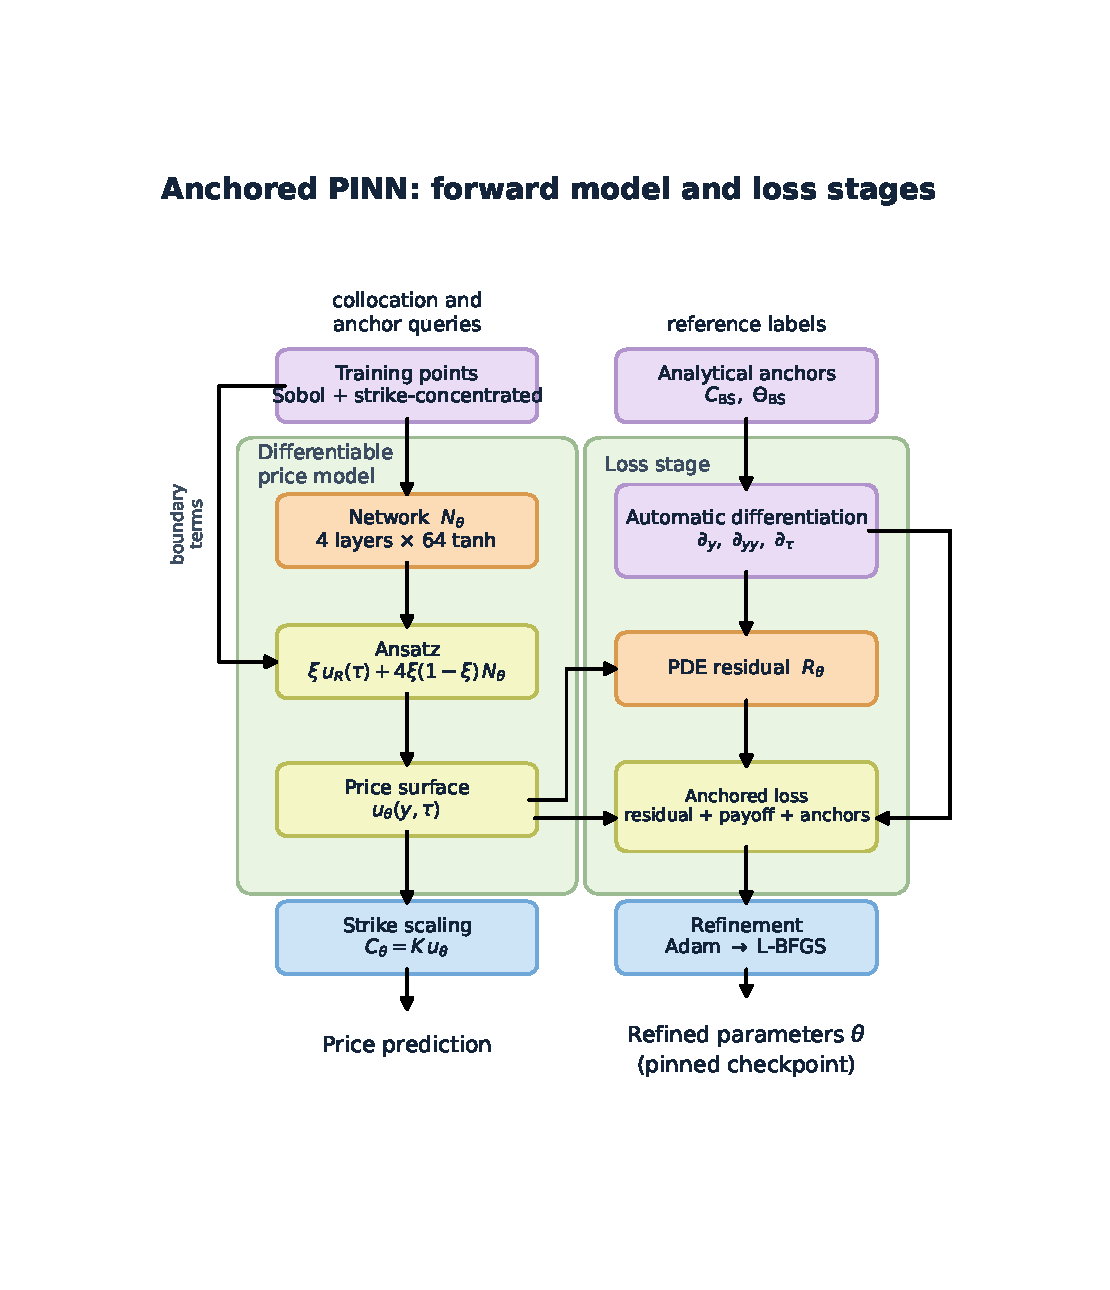
\includegraphics[width=.78\textwidth]{pinn_architecture.pdf}
\caption{The anchored PINN as a two-stage dataflow. Left: the forward model turns Sobol collocation and anchor queries into a boundary-consistent price surface; the routed skip connector injects the boundary terms into the ansatz, bypassing the network. Right: the loss stage differentiates that surface to form the PDE residual and the anchored objective, and the refinement loop returns the updated, checkpoint-pinned parameters.}
\label{fig:pinn-arch}\end{figure}

\subsection{Implementation}
\label{sec:pinn-impl}

The network $N_\theta$ has four hidden layers of 64 tanh units and the whole model runs in float64; double precision reduces roundoff when differentiating quantities on different scales. Collocation and data points are scrambled Sobol sets covering the PDE interior and the payoff boundary, with extra sampling concentrated around the strike, where the payoff kink and the largest Greek curvature live. The initial model is trained with Adam and polished with L-BFGS; the anchored refinement then uses 8,192 analytical price/Theta points with 75\% in the anchor region $S/K\in[0.4,1.6]$, in four staged Adam/L-BFGS passes that successively emphasise price, PDE, and Theta terms of Equation~\eqref{eq:pinn-loss}. The anchor region is wider than the evaluation core. The saved primary checkpoint is identified by a pinned SHA-256 digest in the model registry, so the reported primary metrics refer to that saved artefact.

The metadata separately records 3,002.8 seconds for initial training, 1,008.4 seconds for subsequent refinement, and 1,378.6 seconds for anchored refinement (about 89.8 minutes when summed). These stage records are reported separately in Section~\ref{sec:res-cost}; they are not a single end-to-end timing run. Warm inference evaluates price, Delta, Gamma, and Theta together at roughly $4.6\times10^4$ points per second in batches of 4,096. A comparable workload is needed before this throughput can support an amortisation claim.

\subsection{Evaluation protocol}
\label{sec:pinn-eval}

Evaluation uses a $161\times51$ moneyness--maturity grid over the full training domain. The accuracy region is $S/K\in[0.5,1.5]$ and $\tau\ge0.05$ (1,920 points); a separate full-grid check records negative prices, invalid Delta bounds, and negative Gamma, with an absolute tolerance of $10^{-5}$ in each quantity's units. Greeks at the payoff kink are excluded. This protocol makes a low price RMSE insufficient by itself to declare the model financially admissible: the accuracy gates measure average error within the trained region, while shape checks test financial constraints at the sampled grid points; they do not prove validity between those points.

\section{Deep Operator Networks for Cross-Contract Pricing}
\label{sec:deeponet}

The anchored PINN of Section~\ref{sec:pinn} fixes the rate, dividend yield, and volatility. Changing those coefficients requires a new solution. Strike changes alone can be represented by $C=K u(\log(S/K),\tau)$ within the trained moneyness and maturity domain. The DeepONet additionally learns variation across the model coefficients. This section develops the two DeepONet architectures compared in this report --- an unconstrained control and a parity-constrained model --- and the matched protocol that makes their comparison meaningful. Earlier checkpoint families (a price-only pilot and a Greek-focused $\lambda=1$ model) are retained only as references and are not the comparison models here.

\subsection{Operator-learning formulation}
\label{sec:deeponet-theory}

Where the PINN approximates one function $u(y,\tau)$, a DeepONet approximates an operator: a mapping $G$ that sends contract parameters $a$ to an entire price surface $G(a)\colon(S,\tau)\mapsto V$. The universal approximation theorem for operators \cite{chen1995} justifies the search for such a $G$, and the DeepONet architecture \cite{lu2021} realises it with two subnetworks whose outputs are combined by an inner product. The branch network encodes the contract input $a=(K,T,r,q,\sigma,\mathrm{type})$ into coefficients $b_k(a)$; the trunk network encodes the evaluation coordinate $z=(S,\tau)$ into features $t_k(z)$:
\begin{equation}
V_\theta(a;S,\tau)=K\left[\frac{1}{\sqrt p}\sum_{k=1}^{p}b_k(a)\,t_k(S,\tau)+b_0\right],\qquad p=64 .
\label{eq:deeponet}
\end{equation}
The outer scaling by $K$ reflects the positive homogeneity of Black--Scholes prices in $(S,K)$: the learned target is a dimensionless price, and the physical price is recovered by one multiplication. This is the same strike normalisation used in the loss below.

The trunk can be viewed as learning a collection of reusable shapes; the branch chooses their coefficients for each contract. This resembles an expansion in basis functions, except that both the shapes and the coefficient map are learned. The operator-approximation results underlying DeepONet establish representational possibilities under compactness and continuity assumptions \cite{chen1995,lu2021}. They do not guarantee monotonic improvement from increasing rank in a finite training run.

Our branch receives a finite parameter vector rather than samples of an arbitrary input function. The model is therefore a DeepONet-style \emph{parametric solution surrogate}. The trunk actually receives scaled moneyness and remaining time,
\begin{equation}
\widetilde z=\left((S/K-1)/0.3,\ \tau-1\right),
\end{equation}
so it also depends on $K$ through moneyness. Multiplying the output by $K$ scales the target sensibly, but does not enforce exact homogeneity because $K$ is also a branch input. These details distinguish the implemented model from an idealised separable expansion with a contract-independent trunk.

It is helpful to distinguish three sources of error: limited network capacity, incomplete optimisation, and performance on unseen inputs. For any well-defined population loss $\mathcal E$ over a specified input distribution, one can write
\begin{equation}
\mathcal E(\widehat\theta)=\inf_\theta\mathcal E(\theta)
+\left[\mathcal E(\widehat\theta)-\inf_\theta\mathcal E(\theta)\right].
\label{eq:deeponet-error}
\end{equation}
The first term is the best error the chosen function class could attain. The remaining gap reflects how data and optimisation produced the particular fitted model; the experiment does not identify those effects separately. Validation measures this behaviour on held-out samples. Analytical labels remove market noise from the targets, but do not remove finite-data error, numerical roundoff, or optimisation difficulty. Physics-informed DeepONets add a PDE loss \cite{wang2021}; our DeepONets instead learn from analytical prices and Greeks.


\subsection{Control and parity architectures}
\label{sec:deeponet-arch}

The ordinary \emph{control} network learns calls and puts as one function family, separated by the option-type feature in the branch. Nothing in its output ties the two branches of the family together, so its call and put predictions can violate put--call parity, Equation~\eqref{eq:parity}, by an arbitrary amount at any input.

The \emph{parity} architecture enforces the identity structurally (Figure~\ref{fig:deep-schematic}). Its branch drops the option-type feature, and the network learns only their shared midpoint $M_\theta$; the two prices are then reconstructed from the \emph{analytically known} difference
\begin{equation}
C_\theta=M_\theta+\tfrac12D,\qquad
P_\theta=M_\theta-\tfrac12D,\qquad
D=Se^{-q\tau}-Ke^{-r\tau}. \label{eq:parity-deeponet}
\end{equation}
It follows that $C_\theta-P_\theta=D$ to numerical precision for every input, for every contract, in both training and deployment --- the parity relation is a property of the architecture, not of the optimiser's success. The construction has one deliberate limitation: it guarantees exactly the identity it encodes. Positivity of the reconstructed prices, the call bounds $0\leq\Delta_C\leq e^{-q\tau}$ and put bounds $-e^{-q\tau}\leq\Delta_P\leq0$, and convexity (nonnegative Gamma) are \emph{not} enforced, so parity errors are eliminated while shape violations can remain --- a distinction the results bear out.

\begin{figure}[htbp]\centering
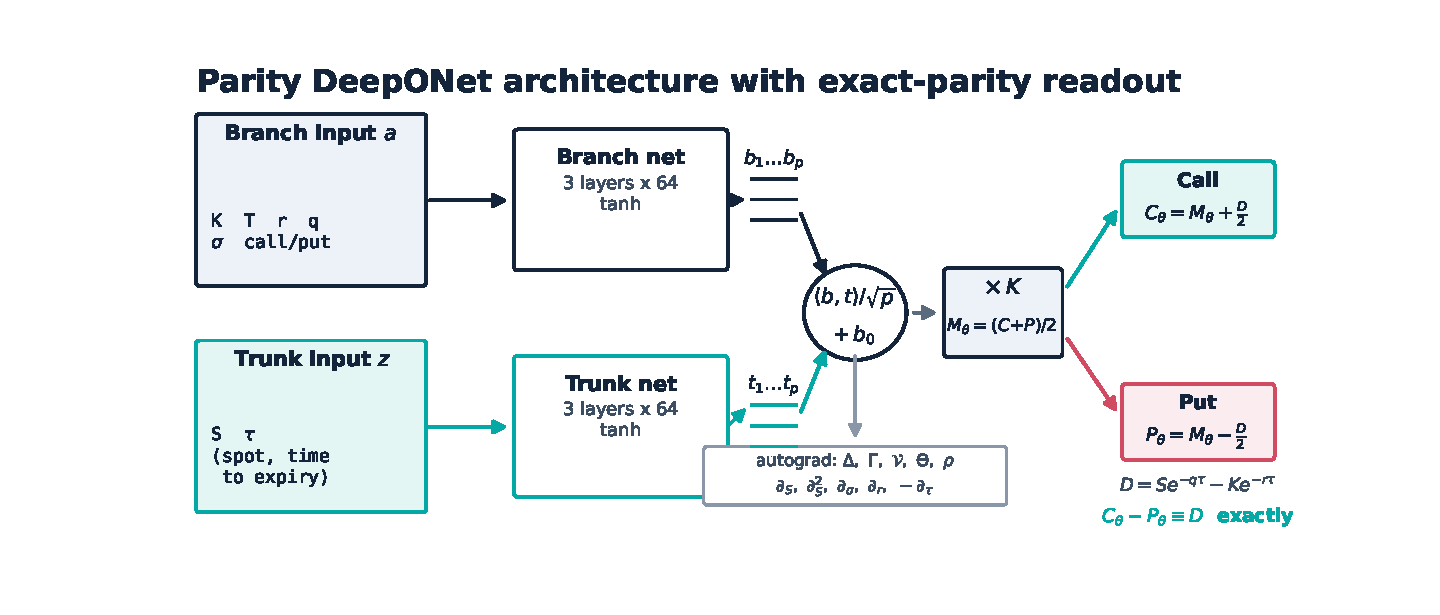
\includegraphics[width=.98\textwidth]{deeponet_schematic.pdf}
\caption{The parity DeepONet in the branch--trunk form of \cite{lu2021}. Both networks are three-layer, width-64 tanh multilayer perceptrons with $p=64$ features; the option-type input exists only in the control arm. The exact-parity readout reconstructs the call and put from one learned midpoint and the analytical difference $D$; all reported Greeks are automatic derivatives of the reconstructed prices in the raw input coordinates: $\Delta=V_S$, $\Gamma=V_{SS}$, $\mathcal V=V_\sigma$, $\mathrm{Rho}=V_r$, and calendar $\Theta=-V_\tau$.}
\label{fig:deep-schematic}\end{figure}

The exactness of the readout has sharper consequences than the parity identity alone. Although $D$ depends on branch parameters $K,r,q$, it is affine in $S$ at fixed contract parameters, so the reconstruction contributes no spot curvature: the two reconstructed prices share one learned Gamma, and the Delta shift is exact,
\begin{equation}
\Gamma_C=\Gamma_P=\Gamma_M,\qquad
\Delta_C=\Delta_M+\tfrac12e^{-q\tau},\qquad
\Delta_P=\Delta_M-\tfrac12e^{-q\tau}.
\label{eq:parity-greeks}
\end{equation}
Differentiating $D$ transfers every parity relation of Section~\ref{sec:classical-theory} to the reconstructed prices exactly:
\begin{equation}
\Delta_C-\Delta_P=e^{-q\tau},\qquad
\mathcal V_C=\mathcal V_P,\qquad
\Theta_C-\Theta_P=qSe^{-q\tau}-rKe^{-r\tau},\qquad
\mathrm{Rho}_C-\mathrm{Rho}_P=K\tau e^{-r\tau},
\label{eq:parity-identities}
\end{equation}
together with $\Gamma_C=\Gamma_P$ from Equation~\eqref{eq:parity-greeks}. Thus the model learns one common surface while preserving the known differences between call and put sensitivities. The control must learn these relationships from data. All reported Greeks are differentiated with respect to the original inputs, including the transformations applied inside the networks.

\subsection{What parity guarantees, and what it leaves to learn}
Write $A=Se^{-q\tau}$ and $B=Ke^{-r\tau}$, so that $D=A-B$. The call and put price bounds can be expressed as
\begin{equation}
\max(D,0)\le C\le A,\qquad \max(-D,0)\le P\le B.
\end{equation}
Substituting $C=M+D/2$ and $P=M-D/2$ reduces both pairs of inequalities to
\begin{equation}
\frac{|A-B|}{2}\le M\le\frac{A+B}{2}.
\label{eq:midpoint-bounds}
\end{equation}
Likewise, the call and put Delta bounds are both satisfied when
\begin{equation}
-\tfrac12e^{-q\tau}\le M_S\le\tfrac12e^{-q\tau},
\qquad M_{SS}\ge0
\label{eq:midpoint-shape}
\end{equation}
also enforces convexity of both prices. Our parity readout enforces their difference; it does not impose these restrictions on the learned midpoint. This provides a direct explanation for a result that otherwise appears contradictory: a model may satisfy parity exactly while still producing negative prices or negative Gamma.

\subsection{Training data and objective}
\label{sec:deeponet-data}

Both arms train on the frozen analytical dataset \texttt{black\_scholes\_operator\_v1}: 256 contracts with 8,192 coordinate queries for training and 64 contracts with 2,048 queries for validation, with branch inputs $(K,T,r,q,\sigma,\mathrm{type})$ and trunk inputs $(S,\tau)$. The dataset and its manifest are hash-pinned before training; the 68 common-benchmark contracts of Section~\ref{sec:classical-impl} were excluded from training and selection for the earlier registered-model evaluation, and real market observations are reserved for a later external study. Inputs are scaled to the training domain. The objective combines a strike-normalised price MSE with RMS-normalised Greek MSEs:
\begin{equation}
\mathcal L_{\rm op}=\left\langle\left(\frac{V_\theta-V_{\rm BS}}{K}\right)^2\right\rangle
+\lambda\frac{1}{5}\sum_{g\in\{\Delta,\Gamma,\mathcal V,\Theta,\mathrm{Rho}\}}
\left\langle\left(\frac{g_\theta-g_{\rm BS}}{s_g}\right)^2\right\rangle,
\label{eq:deep-loss}
\end{equation}
where $s_g$ is the RMS of the corresponding training label, computed from training data only. Dividing by $s_g$ prevents a large numerical unit from dominating simply because of its scale. It does not make every Greek equally difficult or force their gradients to balance. The parameter $\lambda$ controls the relative emphasis on prices and derivatives. Greek supervision asks the network to fit the slopes and curvature of the price function as well as its values; the derivative-error example above explains why that extra information can help.

The single loss weight $\lambda$ trades price accuracy against Greek accuracy, and it is one of the training choices investigated empirically. Table~\ref{tab:weight-sweep} shows the pilot sweep: every tested weight passes the pre-set price gate, the Greek score mildly favours $\lambda=1$, and price error rises monotonically in $\lambda$. The project carried the price-oriented $\lambda=0.01$ forward into replication across three seeds, and that replicated configuration is one parent of the matched comparison below; the $\lambda=1$ model is retained as a Greek-focused reference only. One structural redundancy is recorded here and left unfixed: the branch input contains the contractual maturity $T$ although a time-homogeneous Black--Scholes solution depends on $\tau=T-t$ alone, so the network may learn a spurious dependence on that feature; removing it is a proposed future ablation.

\begin{table}[!ht]\centering\small
\caption{Greek-loss weight sweep on the pilot continuation (300 CPU seconds per arm, fixed dataset). The Greek score averages the five RMS-normalised Greek RMSEs; the training loss averages their squares; all arms pass the pre-set price gate of $0.2157$. The sweep's Greek score favours $\lambda=1$, which is retained as a reference; the price-oriented $\lambda=0.01$ was replicated across seeds and is used in the comparison models.}
\label{tab:weight-sweep}
\begin{tabular}{lrrl}\toprule
Weight $\lambda$ & Price RMSE & Greek score & Price gate\\\midrule
0.01 & 0.183 & 0.0147 & pass\\
0.1  & 0.209 & 0.0164 & pass\\
1    & 0.211 & 0.0128 & pass\\\bottomrule
\end{tabular}\end{table}

\subsection{Matched refinement and selection protocol}
\label{sec:deeponet-protocol}

The comparison of Section~\ref{sec:results} isolates a single factor --- the parity construction --- by holding everything else fixed. The control and parity parents use the same uniform training samples, the same update counts, and three matched seeds; each then receives the same two refinement arms, a 180-second small-step Adam arm and a 180-second full-batch L-BFGS arm, under the same selection rule. Selection retains only candidates whose five Greek RMSEs are within 10\% of their parent, and among those minimises validation price RMSE. Across the six architecture--seed combinations, Adam was selected twice and L-BFGS four times: each architecture selected Adam for one seed and L-BFGS for two. Both optimisers are therefore represented. Matching parent update counts and refinement time caps does not imply identical computation or refinement update counts.

Training and validation data determined the selected checkpoints. The fresh in-domain and broader stress sets were opened afterwards, so they were independent of those selection decisions. They are now observed and cannot serve as untouched tests for later model changes. The earlier 68-contract benchmark has also been observed: its saved results concern the registered $\lambda=0.01$ checkpoint, not the refined parity candidate. This report reads the saved results without rerunning that benchmark. A future comparison of the refined models against the classical methods should specify fresh cases before evaluating them.

\subsection{Why train a surrogate at all? The amortisation argument}
\label{sec:deeponet-amortise}

The motivation for operator learning is \emph{amortisation}: pay a large one-off cost to make every later query cheap. The trade-off is easy to state as a formula. Let $C_{\rm train}$ be the full cost of producing a trained model --- architecture search, training, and label generation included --- let $c_{\rm eval}$ be the marginal cost of one neural query, and let $c_{\rm solve}$ be the cost of answering the same query classically. After $Q$ queries, the surrogate is cheaper when
\begin{equation}
Q \;>\; Q^*\;=\;\frac{C_{\rm train}}{\,c_{\rm solve}-c_{\rm eval}\,},
\qquad c_{\rm solve}>c_{\rm eval}.
\label{eq:breakeven}
\end{equation}
The case for the surrogate thus rests on two numbers that are easy to state and hard to measure honestly. For Black--Scholes vanilla options $c_{\rm solve}$ is minuscule --- the formula is a handful of arithmetic operations --- so $Q^*$ is enormous and amortisation is implausible; the argument becomes interesting only where the classical solve itself is expensive, such as the higher-dimensional problems of Section~\ref{sec:future}. Our timing measurements (Section~\ref{sec:res-cost}) deliberately do not put $C_{\rm train}$ and $c_{\rm solve}$ on a matched footing, so this report claims no numerical break-even point; Equation~\eqref{eq:breakeven} is stated because any future timing comparison should be designed to fill it in.

\section{Results}
\label{sec:results}
All RMSEs below compare each prediction with its analytical Black--Scholes value; the RMSE (root-mean-square error) is the typical size of that gap across the evaluation cases. Prices, Vega, Theta, and Rho are in currency-based units; Delta and Gamma use their usual derivative units, so columns are read down, never across. A ratio of RMSEs is compared only when both methods use the same evaluation set.

For predictions $\widehat f_i$ and reference values $f_i$, we report
\begin{equation}
\operatorname{RMSE}(f)=\sqrt{\frac{1}{n}\sum_{i=1}^{n}(\widehat f_i-f_i)^2}.
\end{equation}
It weights larger errors more heavily than a mean absolute error. A low RMSE can still conceal a small set of poor predictions, so maximum errors, regional plots, and financial checks accompany it. For repeated neural seeds, a mean RMSE averages the separately calculated run-level RMSEs; it is not the RMSE of an ensemble prediction.

\subsection{Classical benchmarks}
\label{sec:res-classical}
The frozen 68-contract set contains 16 anchor, 32 interpolation, and 20 one-parameter extrapolation cases, balanced between calls and puts. An eight-case QuantLib 1.43 cross-check differs from the analytical references by at most $1.09\times10^{-4}$ in price, so the two independent implementations agree. Table~\ref{tab:classical} gives full-set errors, and Figure~\ref{fig:classical-matrix} shows the same data as an error map in which neither method is uniformly dominant: the Crank--Nicolson price error is far below that of RQMC, while RQMC has smaller Gamma and Theta RMSEs on the same cases.

\begin{table}[htbp]\centering\small
\caption{RMSE on 68 common benchmark cases. The conditional RQMC estimate includes its independent pilot and uses 64 scrambles.}
\label{tab:classical}
\begin{tabular}{lrrrrrr}\toprule
Method & Price & Delta & Gamma & Vega & Theta & Rho\\\midrule
Conditional RQMC & $4.7\cdot10^{-5}$ & $7.0\cdot10^{-7}$ & $3.8\cdot10^{-8}$ & $1.1\cdot10^{-4}$ & $3.2\cdot10^{-5}$ & $4.7\cdot10^{-5}$\\
Crank--Nicolson & $1.7\cdot10^{-9}$ & $2.8\cdot10^{-9}$ & $6.8\cdot10^{-7}$ & $9.5\cdot10^{-5}$ & $1.4\cdot10^{-4}$ & $7.8\cdot10^{-6}$\\\bottomrule
\end{tabular}\end{table}
\begin{figure}[htbp]\centering
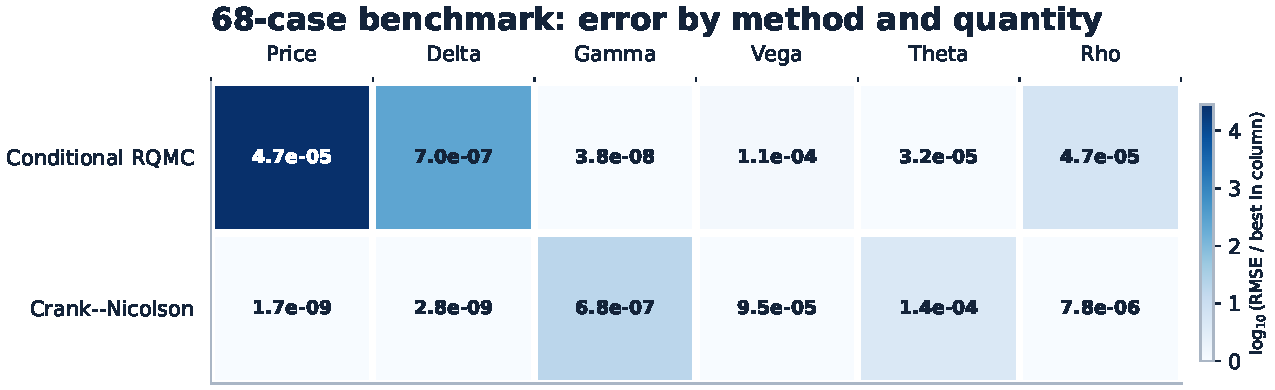
\includegraphics[width=.96\textwidth]{classical_error_matrix.pdf}
\caption{A numerical error map across methods and quantities on the same 68 cases. Cell labels show absolute RMSE. Colour encodes the logarithm of RMSE divided by the smaller RMSE in that column, so unlike physical units are not compared across columns.}
\label{fig:classical-matrix}\end{figure}

Figure~\ref{fig:classical-conv} shows convergence on log--log axes \cite{glasserman2004,rou2025}. Plain Monte Carlo has pooled price exponent $\alpha=0.509$ in ${\rm RMSE}\propto N^{-\alpha}$ across $N=2^{10},\ldots,2^{20}$; eight-scramble Sobol reaches $0.916$, and Sobol with an independently piloted control variate reaches $1.154$, including pilot work. These are empirical slopes for four one-dimensional vanilla contracts. For Crank--Nicolson, joint space--time refinement on uniform grids gives median fitted order $2.000$ across eight cases; the high-volatility put is nonmonotone at finer grids, so this median is not a guarantee for every case. The clustered-mesh Richardson study gives median fitted order $4.00$ using its first three refinement levels, and maximum production-grid price error $3.5\times10^{-9}$ across those eight cases. Its mesh differs from the uniform-grid series, so the plotted error reduction cannot be attributed to extrapolation alone.

\begin{figure}[!t]\centering
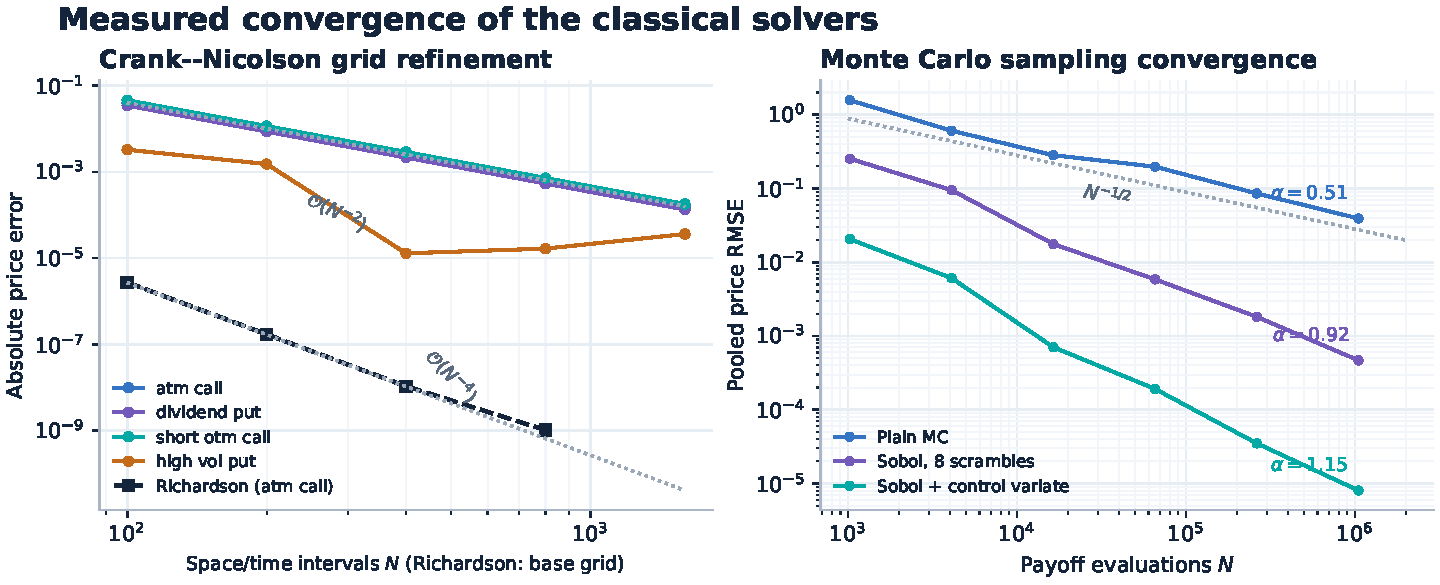
\includegraphics[width=.98\textwidth]{classical_convergence.pdf}
\caption{Measured convergence. Left: uniform-grid Crank--Nicolson for four validation cases, plus the clustered-mesh Richardson series for the ATM call. Space and time are refined together; $N$ denotes the base grid interval count for Richardson. Dotted lines are second- and fourth-order reference slopes. Right: pooled Monte Carlo price RMSE for total payoff budgets $2^{10}$ to $2^{20}$ (24 repetitions per configuration). The controlled estimator allocates half of its total budget to an independent pilot; empirical exponents are annotated.}
\label{fig:classical-conv}\end{figure}

In the separate direct-payoff Greek study, the 32-scramble Sobol-control hybrid estimator on the held-out \texttt{final\_itm\_put} case covered analytical Delta, Theta, and Rho in 19/32, 24/32, and 12/32 repetitions (59\%, 75\%, and 38\%) with nominal 95\% intervals. This result concerns that estimator and case, not the conditional RQMC method in Table~\ref{tab:classical}. The separate conditional high-compute validation records a minimum observed coverage of 89.84\% across its case--quantity checks; passing its screening rule does not establish exact 95\% calibration. Small point-estimate RMSE alone is not evidence of reliable uncertainty.

\subsection{Anchored PINN}
\label{sec:res-pinn}
The fixed-contract anchored PINN passes all registered core accuracy gates (Table~\ref{tab:pinn}). Figure~\ref{fig:pinn-loss} shows the recorded final Theta-anchor stage, with each component multiplied by its training weight. At the last recorded evaluation, Theta accounts for 76.2\% of the weighted objective, the PDE residual 19.6\%, the payoff term 3.6\%, and price 0.6\%. The unweighted PDE residual MSE is about $1.27\times10^{-5}$. This training history documents the final data-assisted refinement; it does not isolate a causal benefit from any one loss term.

\begin{table}[!ht]\centering
\caption{Anchored PINN core-grid RMSE, 1,920 points, against frozen acceptance limits.}
\label{tab:pinn}
\begin{tabular}{lrr}\toprule
Quantity & RMSE & Limit\\\midrule
Price & 0.00980 & 0.020\\
Delta & 0.00247 & 0.010\\
Gamma & 0.000872 & 0.001\\
Theta & 0.0874 & 0.100\\
PDE residual & 0.00333 & 0.010\\\bottomrule
\end{tabular}\end{table}

\begin{figure}[!ht]\centering
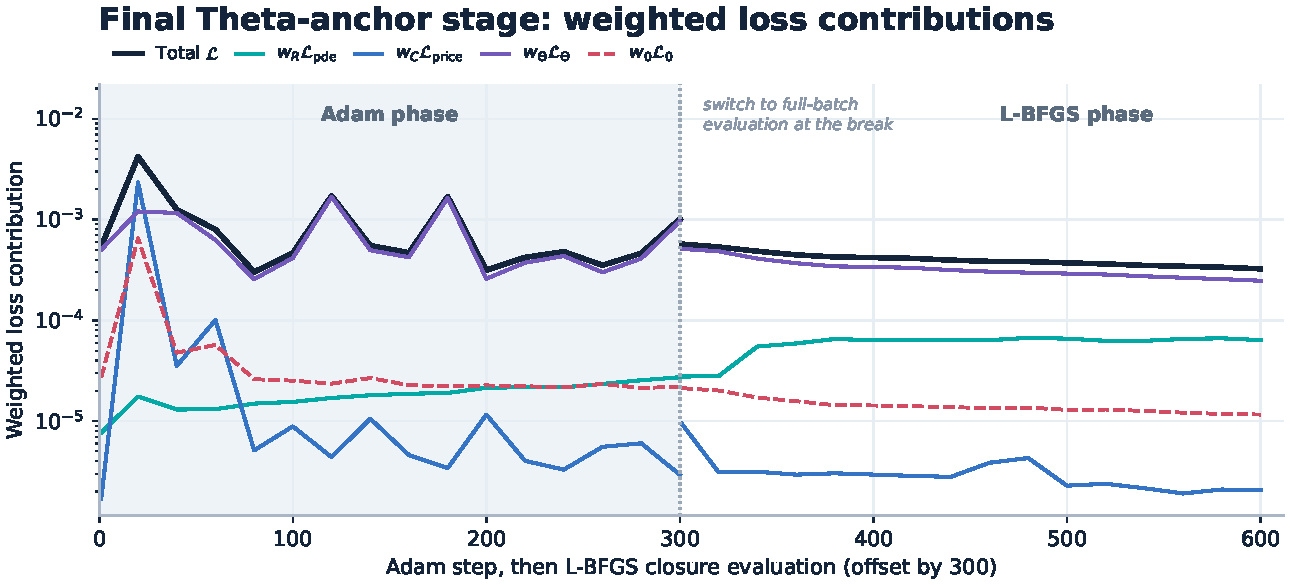
\includegraphics[width=.88\textwidth]{pinn_loss_history.pdf}
\caption{Weighted loss contributions in the recorded final Theta-anchor stage: $w_R=5$, $w_C=100$, $w_\Theta=100$, and $w_0=25$. The components sum to the total at every logged point. The first segment counts Adam steps; the second counts L-BFGS closure evaluations, offset by 300. Adam uses anchor mini-batches of 1,024 points; L-BFGS uses the full 8,192-point anchor set, so changes across the boundary also reflect a change in the evaluation sample. This plot covers the last of four anchored stages. Spatial boundary conditions are embedded, so no boundary-loss curve is needed.}
\label{fig:pinn-loss}\end{figure}

Figure~\ref{fig:pinn-profiles} compares price and its automatic derivatives with the analytical solution. At $\tau=0.06$ the price traces nearly overlap at the displayed scale, with errors of a few cents, but the derivative discrepancies remain visible. Predicted Gamma is positive near the peak ($0.9<S/K<1.1$), while small negative values occur away from the strike, including $S/K\approx1.28$--$1.48$ (inset). Figure~\ref{fig:pinn-surfaces} compares the price surfaces and displays the remaining error on a logarithmic scale. Figure~\ref{fig:pinn-atlas} maps accuracy and shape failures over maturity. Across the full $161\times51$ grid, 700 prices, 609 Deltas, and 3,001 Gammas fall below their lower bounds by more than $10^{-5}$; 2,925 Deltas exceed the upper bound by that tolerance. Even inside the passing core region, 243 of 1,920 points show negative Gamma and 148 show negative prices beyond tolerance. The primary model satisfies the accuracy gates but fails financial shape checks both inside and outside the core.

\begin{figure}[!t]\centering
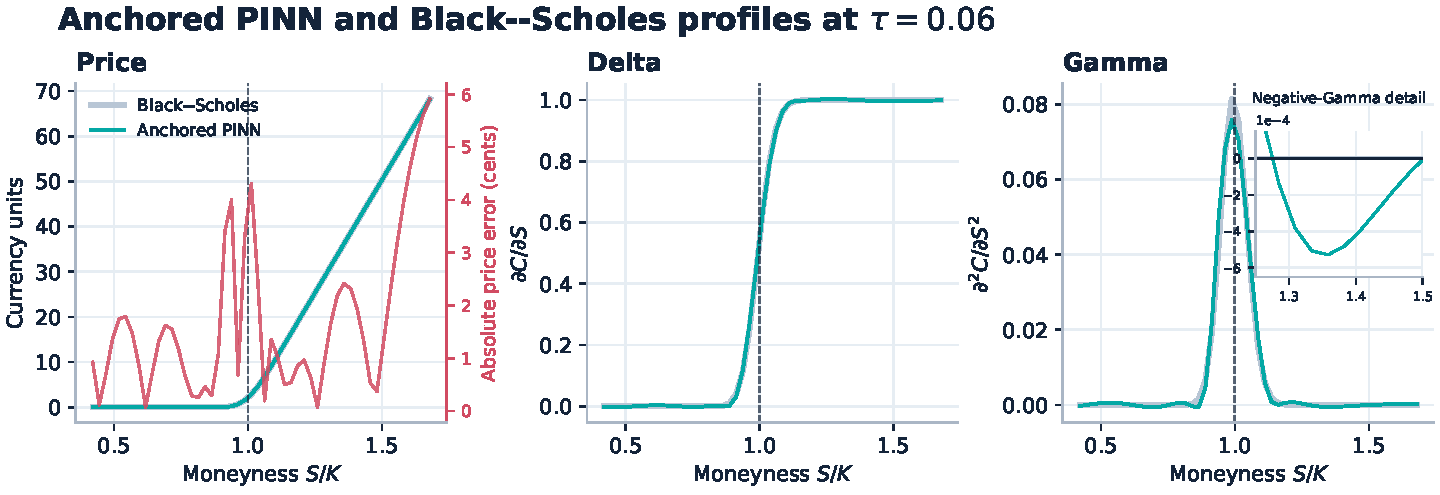
\includegraphics[width=.98\textwidth]{pinn_greeks_profiles.pdf}
\caption{Anchored PINN (teal) against analytical Black--Scholes (grey) at $\tau=0.06$, $K=100$. Left: the price matches to within a few cents (red axis). Middle and right: Delta and Gamma are automatic derivatives of the same price network. The inset magnifies negative Gamma away from the strike; Gamma remains positive around its main peak.}
\label{fig:pinn-profiles}\end{figure}

\begin{figure}[!t]\centering
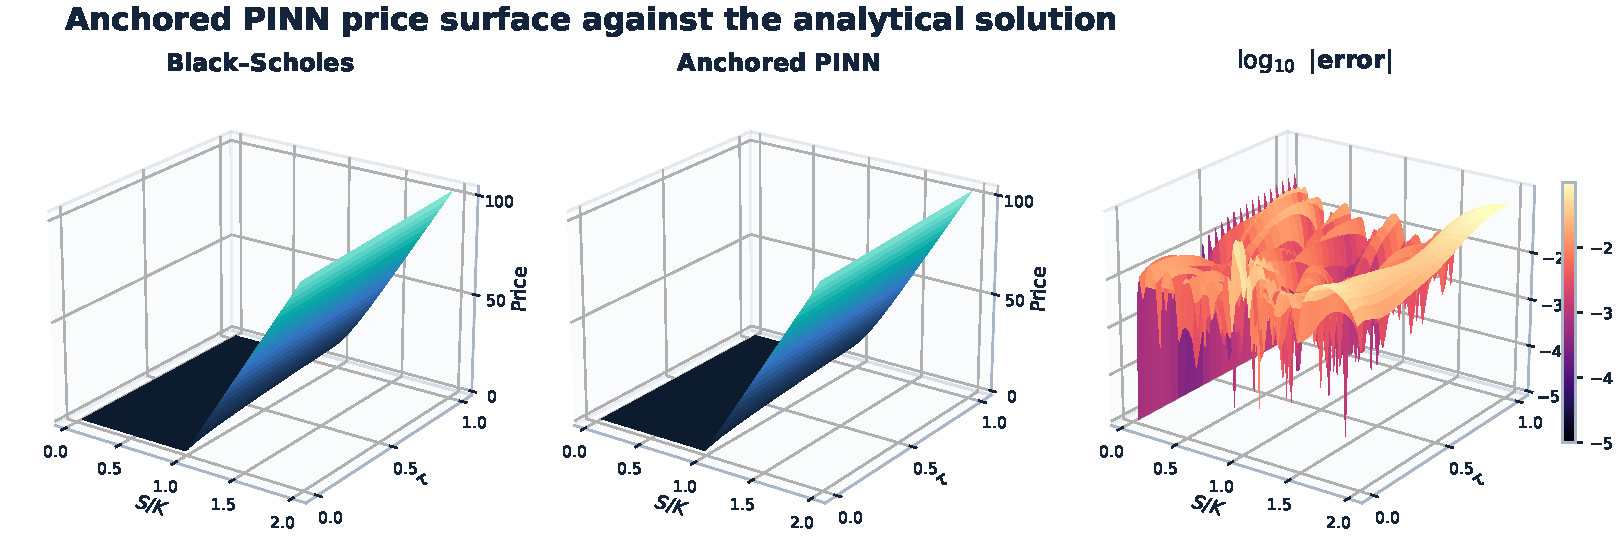
\includegraphics[width=.98\textwidth]{pinn_surfaces.pdf}
\caption{Anchored PINN price surface over moneyness and time to maturity (displayed range $S/K\in[0.05,2]$). The trained surface is visually indistinguishable from the analytical Black--Scholes surface; the log-scale error surface shows the remaining deviations concentrating along the strike at short maturities and in the far in-the-money, long-dated corner (floor at $10^{-5}$, as in Figure~\ref{fig:pinn-atlas}).}
\label{fig:pinn-surfaces}\end{figure}

\begin{figure}[!t]\centering
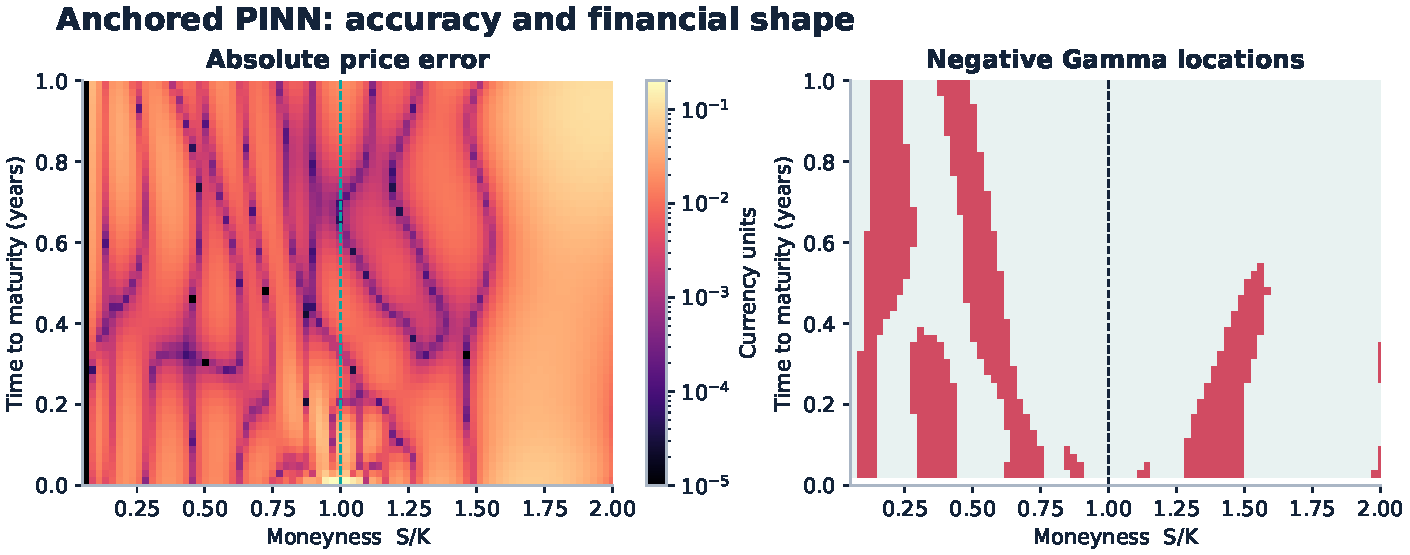
\includegraphics[width=.90\textwidth]{pinn_error_atlas.pdf}
\caption{Anchored PINN on the fixed-contract surface. Left: absolute price error on a log colour scale; right: locations with Gamma below $-10^{-5}$. The dashed line marks at-the-money. The displayed moneyness range is $[0.05,2]$ for legibility; shape counts refer to the full $[0.05,4]$ grid.}
\label{fig:pinn-atlas}\end{figure}

\subsection{Registered DeepONet on the held-out benchmark}
\label{sec:res-deep-benchmark}
The registered DeepONet primary --- the replicated $\lambda=0.01$ control evaluated once on the 68-contract benchmark before the parity study was designed --- has price RMSE 0.276 and maximum absolute price error 1.298 across all cases. The split rows of Table~\ref{tab:deep-benchmark} localise the error: 0.093 on the anchor cases, 0.133 on interpolation, and 0.473 on the one-parameter extrapolation cases, a $3.6\times$ degradation. Vega and Rho both deteriorate out of domain (Vega 0.70 to 3.97; Rho 1.22 to 5.69); the pooled split does not by itself identify which parameter excursions cause these errors; the anchor split carries the largest Theta error (2.27), driven by short-maturity cases where Theta is large and steep. This once-measured benchmark is reported as the only number tied to the registered checkpoint; the parity comparison below uses its own validation and fresh sets, and the two protocols are not pooled.

\begin{table}[!ht]\centering\small
\caption{Registered DeepONet ($\lambda=0.01$ control) on the one-time 68-contract benchmark: RMSE by benchmark split. This evaluation predates the parity study and has not been repeated.}
\label{tab:deep-benchmark}
\begin{tabular}{lrrrrrrl}\toprule
Split (cases) & Price & Delta & Gamma & Vega & Theta & Rho & Max price error\\\midrule
All (68) & 0.276 & 0.0162 & 0.00232 & 2.24 & 1.23 & 3.25 & 1.30\\
Anchor (16) & 0.093 & 0.0123 & 0.00148 & 0.83 & 2.27 & 1.26 & 0.19\\
Interpolation (32) & 0.133 & 0.0101 & 0.00155 & 0.70 & 0.34 & 1.22 & 0.34\\
Extrapolation (20) & 0.473 & 0.0246 & 0.00357 & 3.97 & 0.90 & 5.69 & 1.30\\\bottomrule
\end{tabular}\end{table}

\subsection{Parity versus matched control}
\label{sec:res-parity}
The refined parity candidate was developed after the benchmark evaluation above, so its 0.066 validation RMSE cannot be directly compared with the registered benchmark figure. Table~\ref{tab:deep} instead compares parity against its contemporaneous, matched control over three seeds. Parity reduces all six mean validation RMSEs, and each paired seed improves in price: Figure~\ref{fig:deep-paired} shows the three paired seed trajectories on the validation, fresh in-domain, and fresh stress splits. Parity also reduces the observed seed-to-seed spread: its three-seed validation price-RMSE SD is about 17 times smaller than the control's, although three seeds cannot establish general training stability.

\begin{table}[!ht]\centering\small
\caption{Validation RMSE, mean $\pm$ sample SD over three matched seeds. The parity architecture is a candidate; the registered primary is unchanged.}
\label{tab:deep}
\begin{tabular}{lrrr}\toprule
Quantity & Refined control & Refined parity & Change\\\midrule
Price & $0.0913\pm0.0130$ & $0.0660\pm0.0007$ & $-27.7\%$\\
Delta & $0.01063\pm0.00179$ & $0.00838\pm0.00065$ & $-21.1\%$\\
Gamma & $0.002722\pm0.000364$ & $0.002456\pm0.000059$ & $-9.8\%$\\
Vega & $1.000\pm0.035$ & $0.825\pm0.044$ & $-17.4\%$\\
Theta & $1.351\pm0.216$ & $1.117\pm0.072$ & $-17.4\%$\\
Rho & $1.145\pm0.144$ & $1.030\pm0.017$ & $-10.1\%$\\\bottomrule
\end{tabular}\end{table}

\begin{figure}[!ht]\centering
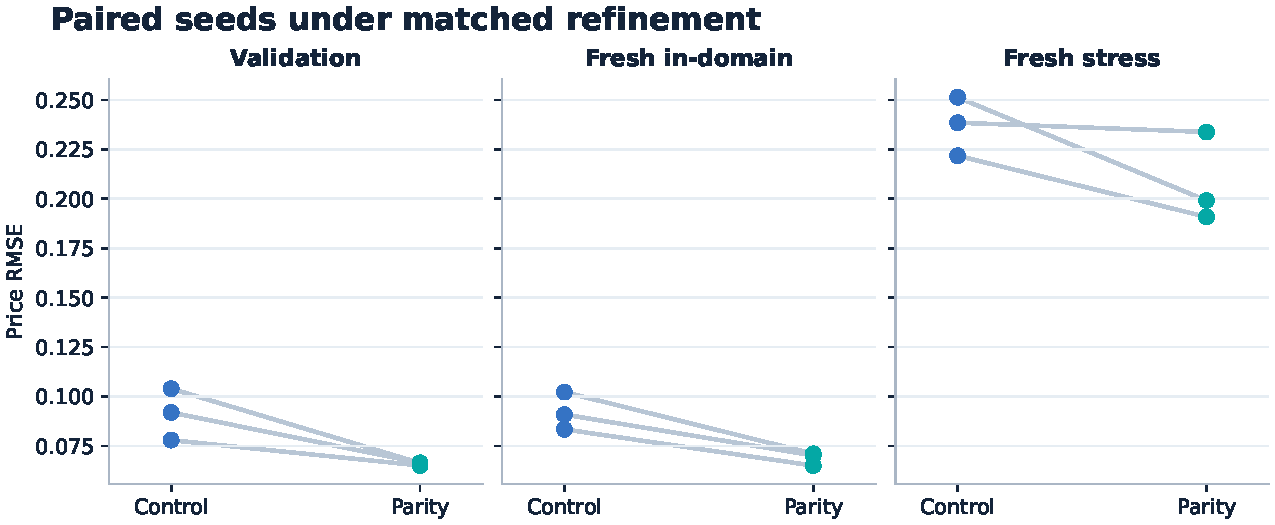
\includegraphics[width=.98\textwidth]{deeponet_paired_seeds.pdf}
\caption{Paired seeds under matched refinement. Each line connects one seed's control and parity price RMSE; every pair improves with parity, on all three evaluation splits.}
\label{fig:deep-paired}\end{figure}

A pooled mean does not reveal the regional distribution of error, so Figure~\ref{fig:deep-regional} stratifies the validation price RMSE by moneyness and remaining maturity, in the spirit of the per-region error reporting used in operator-learning studies \cite{lee2026}. Parity improves every band: by 24--32\% across moneyness, with the largest gain in the $S/K\ge1.1$ band (which mixes in-the-money calls and out-of-the-money puts), and by 29--33\% at short and long remaining maturities. The worst band for both arms is long remaining maturity $\tau\ge1$, where the control's error roughly doubles relative to the near-the-money band within this validation set. These marginal bands describe associations; they do not isolate price magnitude, maturity sensitivity, or distance from the training domain as causes.

\begin{figure}[!ht]\centering
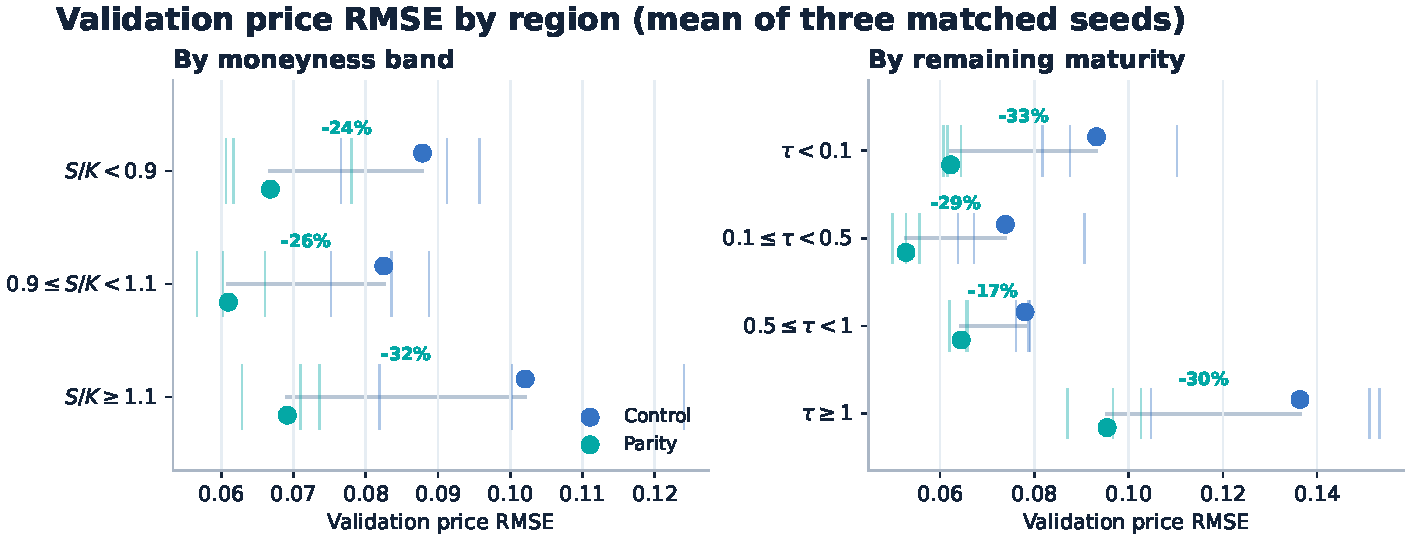
\includegraphics[width=.98\textwidth]{deeponet_regional_errors.pdf}
\caption{Validation price RMSE by region for the refined control (blue) and parity (teal) models: filled dots are three-seed means, faint ticks the individual seeds, and annotations the mean change. Parity improves every band.}
\label{fig:deep-regional}\end{figure}

Figure~\ref{fig:deep-profile} summarises the same comparison as percentage changes across all six quantities and splits: fresh in-domain results agree with validation, and gains narrow on the broader stress set (price 0.237 to 0.208) but stay positive. On the same stress set, the mean price-bound violation frequency is 12.08\% for control and 13.41\% for parity; negative-Gamma frequencies are 13.88\% and 15.19\%, respectively. Frequencies use a $10^{-8}$ absolute tolerance in each quantity's units. Severity does not always move with frequency: the worst price-bound violation across all three seeds decreases from 1.839 to 1.556 currency units, whereas the worst negative-Gamma magnitude increases from 0.0280 to 0.0308. Exact parity therefore does not guarantee admissible prices or convexity. The stress price RMSE remains about three times its in-domain RMSE (0.208 versus 0.0688). An exact financial identity therefore helps the observed mean accuracy while leaving material derivative and extrapolation weaknesses.

\begin{figure}[!t]\centering
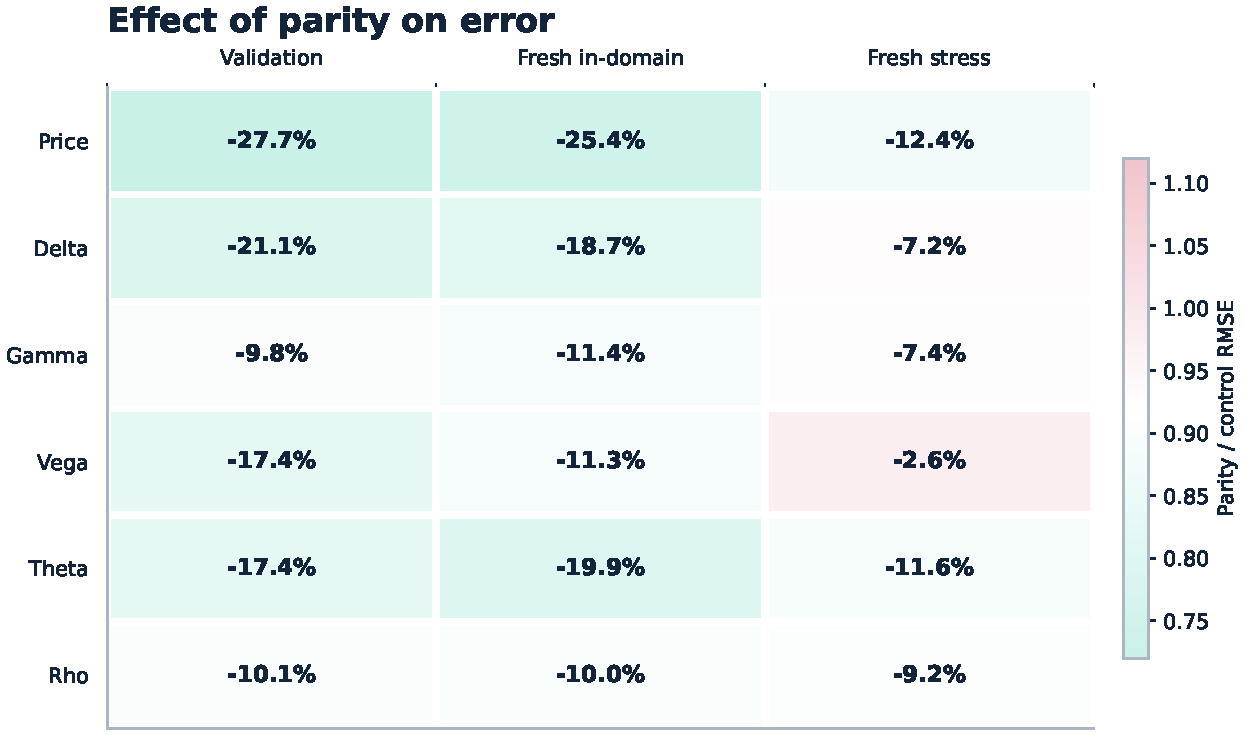
\includegraphics[width=.76\textwidth]{deeponet_error_profile.pdf}
\caption{Percentage change in parity RMSE relative to the matched control; negative values are improvements. ``Stress'' is a wider mixed-domain set, not a pure extrapolation set.}
\label{fig:deep-profile}\end{figure}

\subsection{Earlier computational cost records}
\label{sec:res-cost}
Table~\ref{tab:cost} in Appendix~\ref{sec:reproducibility} collects the detailed runtime records. Classical timing includes price and all five Greeks for batches of six contracts; PINN timing includes price, Delta, Gamma, and Theta for batches of 4,096 coordinates on a fixed surface. The neural training records and DeepONet refinement caps describe additional workloads. These measurements do not establish comparable per-query marginal costs or a numerical break-even point. Section~\ref{sec:fresh-shared} adds a matched inference comparison. A complete amortisation assessment would also require accuracy targets and the full training and label-generation cost; it is not inferred from these earlier records.



\clearpage
\subsection{A cross-method summary}
\label{sec:res-summary}
Table~\ref{tab:master} collects the available price and Greek RMSEs. Its panels identify the evaluation problem, so a reader can see which rows support a direct comparison. The analytical row is zero by definition because it supplies the labels. The PINN does not take volatility and interest rate as varying inputs, so Vega and Rho were not evaluated in its protocol; missing values are shown as dashes, not zeros.

Read a metric down comparable rows. Raw Price, Gamma, Vega, and other columns have different units, and their numerical sizes do not establish which quantity is harder to predict. The matched DeepONet comparison does support a narrower conclusion: adding parity improves the mean RMSE of each reported quantity on the same data. Accuracy and financial validity remain separate, as the preceding shape checks show. Appendix~\ref{sec:historical-rmse} records additional development models without mixing them into the main comparison.
\begin{table}[!ht]\centering\small\setlength{\tabcolsep}{3pt}
\caption{Price and Greek RMSEs grouped by evaluation set. Neural multi-seed rows report the mean of run-level RMSEs. A dash indicates an unreported quantity.}
\label{tab:master}
\begin{tabular}{lrrrrrr}\toprule
Model & Price & Delta & Gamma & Vega & Theta & Rho\\
\midrule\multicolumn{7}{l}{\textit{A. Common benchmark: 68 contracts}}\\
Analytical reference & 0 & 0 & 0 & 0 & 0 & 0\\
Conditional RQMC & $4.68\times10^{-5}$ & $7\times10^{-7}$ & $3.78\times10^{-8}$ & 0.000114 & $3.2\times10^{-5}$ & $4.74\times10^{-5}$\\
Crank--Nicolson + Richardson & $1.66\times10^{-9}$ & $2.8\times10^{-9}$ & $6.8\times10^{-7}$ & $9.5\times10^{-5}$ & 0.000137 & $7.81\times10^{-6}$\\
DeepONet: registered primary & 0.276 & 0.0162 & 0.00232 & 2.24 & 1.23 & 3.25\\
\midrule\multicolumn{7}{l}{\textit{B. Fixed-call core surface: 1,920 coordinates}}\\
Anchored PINN & 0.0098 & 0.00247 & 0.000872 & --- & 0.0874 & ---\\
\midrule\multicolumn{7}{l}{\textit{C. DeepONet validation: 2,048 queries; three seeds}}\\
Refined DeepONet control & 0.0913 & 0.0106 & 0.00272 & 1 & 1.35 & 1.15\\
Refined DeepONet parity & 0.066 & 0.00838 & 0.00246 & 0.825 & 1.12 & 1.03\\
\midrule\multicolumn{7}{l}{\textit{D. Fresh in-domain: 4,096 queries; three seeds}}\\
Refined DeepONet control & 0.0922 & 0.0107 & 0.00249 & 0.943 & 1.5 & 1.13\\
Refined DeepONet parity & 0.0688 & 0.00869 & 0.0022 & 0.836 & 1.2 & 1.02\\
\midrule\multicolumn{7}{l}{\textit{E. Fresh stress: 2,048 queries; three seeds}}\\
Refined DeepONet control & 0.237 & 0.019 & 0.00362 & 1.95 & 1.99 & 3.08\\
Refined DeepONet parity & 0.208 & 0.0177 & 0.00336 & 1.9 & 1.75 & 2.79\\
\bottomrule\end{tabular}\end{table}




\clearpage
\subsection{Fresh shared evaluation of the frozen models}
\label{sec:fresh-shared}
The earlier studies answered different questions on different datasets. To make a direct comparison, a new set of 512 queries was frozen together with the numerical budgets, checkpoint identities, and evaluation rules before predictions were generated. The fixed-parameter panel contains 256 calls at the PINN's parameters; the cross-contract panel contains 128 market states, each queried as a call and a put. The PINN is excluded from the latter panel. The parity checkpoint was chosen using existing validation results: seed 22092027 had the lowest validation price RMSE among the three previously refined seeds. No new training or test-based checkpoint selection was performed.

Table~\ref{tab:fresh-shared} gives the common-domain results. The fixed-panel subset uses $S/K\in[0.7,1.3]$ and $\tau\in[0.05,1]$, so both neural models are queried within their supported ranges. The anchored PINN has smaller errors than the general-purpose DeepONet on this fixed surface, while the classical numerical solvers are substantially more accurate than either network. This does not show that a fixed PINN is preferable for changing market parameters: it does not solve that broader task.
\begin{table}[!ht]\centering\small\setlength{\tabcolsep}{3pt}
\caption{Fresh common-domain RMSEs. Rows within each panel use exactly the same queries. The fixed PINN supplies four outputs; it is excluded from the cross-contract panel. Analytical errors are zero by definition.}
\label{tab:fresh-shared}
\begin{tabular}{lrrrrrr}\toprule
Method & Price & Delta & Gamma & Vega & Theta & Rho\\
\midrule\multicolumn{7}{l}{\textit{Fixed parameters: 128 calls}}\\
Analytical reference & 0 & 0 & 0 & --- & 0 & ---\\
Conditional RQMC & $2.75\times10^{-5}$ & $8.14\times10^{-7}$ & $6.66\times10^{-8}$ & --- & $5.30\times10^{-5}$ & ---\\
CN + Richardson & $9.09\times10^{-10}$ & $7.37\times10^{-9}$ & $1.68\times10^{-7}$ & --- & $2.78\times10^{-5}$ & ---\\
Anchored PINN & 0.01107 & 0.002865 & 0.001125 & --- & 0.09423 & ---\\
Parity DeepONet & 0.04265 & 0.006023 & 0.001245 & --- & 0.3178 & ---\\
\midrule\multicolumn{7}{l}{\textit{Varying parameters: 128 interpolation queries}}\\
Analytical reference & 0 & 0 & 0 & 0 & 0 & 0\\
Conditional RQMC & $4.55\times10^{-5}$ & $7.71\times10^{-7}$ & $5.25\times10^{-8}$ & 0.0001462 & 0.0001041 & $3.58\times10^{-5}$\\
CN + Richardson & $1.20\times10^{-9}$ & $6.59\times10^{-9}$ & $1.14\times10^{-7}$ & $8.05\times10^{-5}$ & $5.03\times10^{-5}$ & $1.94\times10^{-6}$\\
Parity DeepONet & 0.0742 & 0.006988 & 0.002 & 1.003 & 0.538 & 1.784\\
\bottomrule\end{tabular}\end{table}


The remaining queries make the limits visible. The fixed panel adds 64 moneyness-tail cases and 64 short-maturity cases. The broader panel adds 32 short-maturity and 96 extrapolation queries; its maturity extension changes both $T$ and $\tau$. For the selected parity model, cross-contract price RMSE rises from 0.0742 on interpolation cases to 0.1272 across the full mixture. Near expiry, Greek errors grow much more strongly: fixed-panel short-maturity Theta RMSE is 2.70 for the PINN and 4.47 for DeepONet, and cross-contract short-maturity Theta RMSE is 7.78. These are distribution-specific errors, not changes to the saved models. A visually close price approximation is still insufficient for reliable sensitivities. Across the three parity seeds, full cross-contract price RMSE ranges from 0.127 to 0.204; the small validation spread therefore does not establish general stability outside that validation distribution.

Financial checks use a common absolute tolerance of $10^{-5}$. On all fixed-panel queries, price-bound violations occur at 9.77\% of PINN points and 26.17\% of parity-model points; the latter panel includes tails outside the DeepONet training range. On the broader panel, the selected parity model has price-bound and negative-Gamma violation frequencies of 5.47\% and 7.81\%. The classical methods have no violations beyond tolerance on these sampled cases. The parity model's maximum call--put difference error is about $7.1\times10^{-15}$ on the 128 paired states: its encoded identity holds, but its other financial restrictions do not follow automatically.

\paragraph{Matched inference workloads.}
The new timing runs use CPU float64, two configured numerical-library threads, one warm-up, and five repetitions at batch sizes 1, 8, and 32. Each panel and method runs in a separate process. Input conversion, computation, and output conversion are included; checkpoint loading is excluded. The fixed-panel CN adapter omits unused Vega and Rho bump solves and was checked against the existing full solver. Native conditional RQMC still computes six outputs internally. A global NumPy change interrupted the initial timing series; those partial measurements were archived, and all final timing runs were restarted with the frozen versions checked in every worker.
\begin{table}[!ht]\centering\small
\caption{Fresh timing comparison at batch size 32: median milliseconds per query over five repetitions after one warm-up. The fixed panel requests four outputs and the varying panel six. Detailed repetition spread and memory are retained with the results.}
\label{tab:fresh-timing}
\begin{tabular}{lrr}\toprule
Method & Fixed parameters & Varying parameters\\\midrule
Analytical reference & 0.04511 & 0.01884\\
Conditional RQMC & 384.8 & 352.2\\
CN + Richardson & 158.7 & 729.5\\
Anchored PINN & 0.08329 & ---\\
Parity DeepONet & 0.1585 & 0.1747\\
\bottomrule\end{tabular}\end{table}


\begin{figure}[!ht]\centering
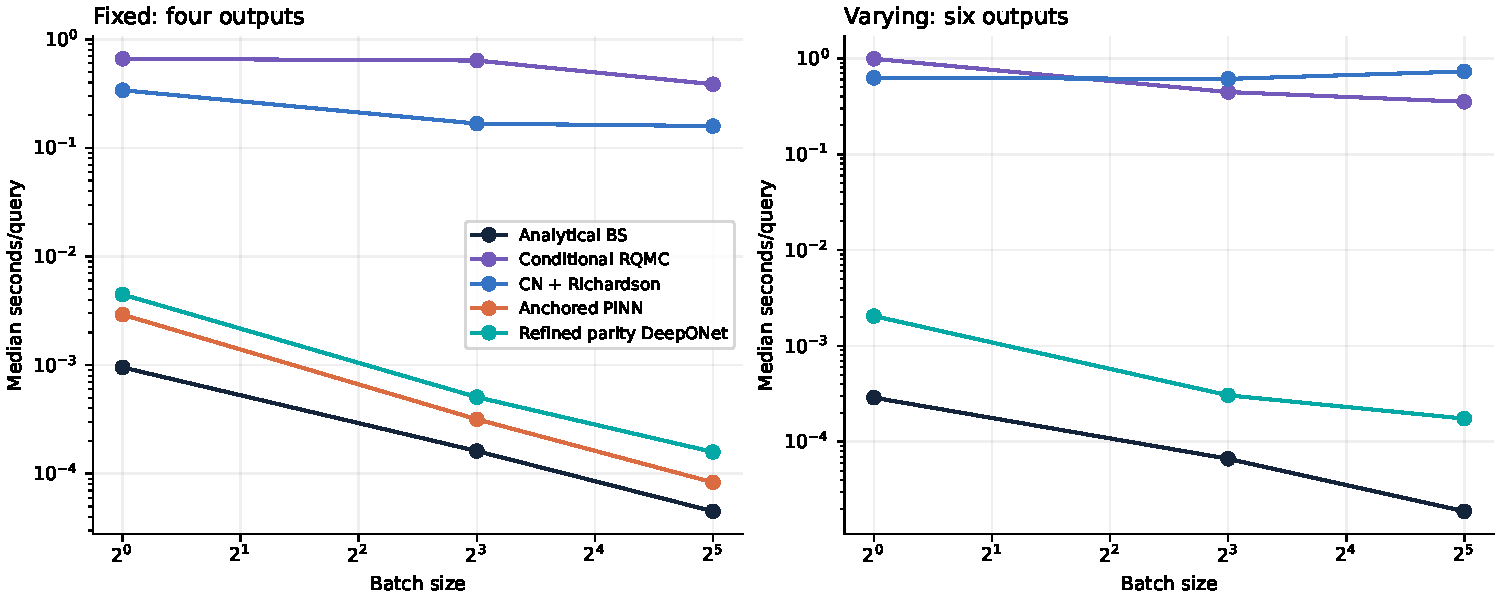
\includegraphics[width=.96\textwidth]{fresh_batch_timing.pdf}
\caption{Median inference cost per query as the batch grows. Workloads are matched within each panel. The numerical solvers answer independent queries; reuse of a cached CN surface is not measured. Faster inference is not an accuracy-matched advantage.}
\label{fig:fresh-timing}\end{figure}

The networks are fast relative to the independent numerical solves, but the analytical formula remains both faster and exact for the stated model. Training and label generation are additional costs. The recorded neural training stages, full regional errors, all three parity seeds, worst cases, timing spread, sampled memory, and integrity checks are retained under \path{results/shared_comparison/v1/}. The new queries are now observed; subsequent model changes require another independent assessment.

\clearpage
\section{Conclusion}
\label{sec:conclusion}
The shared evaluation gives a clear conclusion for the one-dimensional European options studied here: the classical numerical methods achieve smaller price and Greek errors than the frozen neural models. Analytical Black--Scholes remains the simplest reference and the fastest available solution under these assumptions. Crank--Nicolson with Richardson extrapolation and conditional RQMC provide accurate numerical alternatives, although the latter uses analytical continuation and is not independent of the Black--Scholes formula. These findings concern the stated contracts, domains and computational budgets; they do not establish a universal ranking for more complex pricing problems.

The neural models show useful capabilities, with important limits. The anchored PINN closely approximates its fixed-contract surface using both the pricing equation and analytical observations. The parity DeepONet learns across contracts and satisfies the call--put identity by construction. Against its matched neural control, that structure improves the measured price and Greek errors across the three studied seeds. Neither result removes the need for independent checks: short-maturity Greeks remain difficult, and both neural models can violate price bounds or convexity. Accurate prices alone therefore do not establish reliable sensitivities or financially consistent behaviour.

Once trained, the networks answer batches much faster than the independently executed numerical solves at the tested settings. This is an inference-only advantage at unequal errors, not an accuracy-matched or overall computational advantage. Training, analytical label generation, and model selection add costs; the full cost of these stages was not measured under the inference protocol. The experiments also do not measure reuse of a finite-difference surface across related queries. No end-to-end speedup or break-even number of queries is established.

The main contribution of this study is a reproducible comparison that makes these distinctions explicit. The fixed-surface and varying-parameter tasks are evaluated separately, the chosen checkpoints are preserved, and prices, Greeks, financial restrictions and timing are reported together. The evidence supports retaining neural methods as candidates for harder pricing problems, while using the present classical results as the accuracy standard. Future work should test whether their rapid inference becomes useful when an analytical solution is unavailable and a clearly stated accuracy requirement can be met.

\clearpage
\section{Further Work}
\label{sec:future}
The fresh shared comparison now provides a common reference for the frozen models. The next experiments should address specific remaining weaknesses: short-maturity Greeks, financial shape restrictions, and performance outside the training range. Accuracy targets and total computational cost should guide any practical deployment claim. The existing test sets, including the new shared queries, are now observed; further improvements must use validation data for selection and reserve fresh cases for their final assessment.

\begin{itemize}
\item \textbf{More reliable neural prices and Greeks.} Exact parity leaves price bounds and convexity unresolved. A useful next experiment would constrain the learned midpoint using Equations~\eqref{eq:midpoint-bounds}--\eqref{eq:midpoint-shape}, then check whether fewer violations come at an accuracy cost. Sampling near difficult regions and removing the redundant maturity input should be tested separately, with matched seeds and training budgets.
\item \textbf{A market-data case study.} Prices from liquid NSE-listed options could test how the Black--Scholes assumptions compare with market quotes. This is a different question from numerical accuracy: an exact model solution can still disagree with the market. Bid--ask spreads, liquidity filters, and the way volatility is estimated must be stated. Market quotes do not directly provide Greek labels, so Greek quality would need a separate sensitivity or hedging assessment.
\item \textbf{Multi-asset options.} A basket option depends on several correlated asset prices. Beginning with two or three assets would test whether neural methods become more useful as grid-based solvers grow expensive. Conditional RQMC and suitable control variates would provide simulation baselines. Evaluation should include asset-wise Deltas, cross-Gammas, and the total cost of training and repeated use.
\item \textbf{Calibration and early exercise.} Calibration reverses the pricing problem: observed prices are used to infer volatility or other parameters. American options introduce a different challenge, because the holder can exercise before maturity. Both require separate validation: synthetic parameter-recovery tests for calibration, and established early-exercise solvers for American options.
\item \textbf{Richer market models.} Time-varying rates and volatility provide a controlled extension of the constant-coefficient setting. Jump models introduce sudden asset-price changes. Extensions with known analytical or semi-analytical European prices would preserve the ability to measure numerical error before relying on purely numerical references.
\end{itemize}

\clearpage
\appendix
\section{Recorded Experimental Settings}
\label{sec:reproducibility}

This appendix records settings from the saved configurations and metadata. It introduces no new training run or held-out evaluation. All Greek units follow Section~\ref{sec:classical-theory}.

\subsection{Datasets and parameter domains}
The DeepONet training set has 256 contracts and 8,192 queries; validation has 64 contracts and 2,048 queries (32 coordinates per contract in each). The fresh in-domain set has 256 contracts and 4,096 queries; the fresh stress set has 128 contracts and 2,048 queries (16 coordinates per contract). The matched seeds are 22092026, 22092027, and 22092028; fresh-set seeds are 28092026 and 28093026. Both option types are represented. Queries satisfy $\tau\le T$.

\begin{table}[!ht]\centering\small
\caption{DeepONet sampling ranges. Rates and volatility are decimal inputs; times are in years.}
\begin{tabular}{lrr}\toprule
Parameter & Training / fresh in-domain & Fresh stress\\\midrule
$K$ & $[80,120]$ & $[75,125]$\\
$T$ & $[0.05,2]$ & $[0.03,2.5]$\\
$S/K$ & $[0.7,1.3]$ & $[0.6,1.4]$\\
$\sigma$ & $[0.1,0.6]$ & $[0.08,0.65]$\\
$r$ & $[-0.02,0.10]$ & $[-0.03,0.12]$\\
$q$ & $[0,0.06]$ & $[0,0.08]$\\
Minimum $\tau$ & $0.01$ & $0.005$\\\bottomrule
\end{tabular}\end{table}

The separate 68-case benchmark fixes $K=100$ and retains its original 16/32/20 anchor/interpolation/extrapolation labels. Its interpolation envelope uses $\tau\in[0.05,2]$, with the same moneyness, volatility, rate, and dividend ranges as the training column above. These frozen categories should not be confused with the wider mixed-domain fresh stress set.

\subsection{Classical solver budgets}
Conditional RQMC uses 64 independent scrambles, each with 4,096 production points and 2,048 pilot points, conditional fraction $c=0.25$, and independent pilot control coefficients. The total is 393,216 simulated states per contract. Crank--Nicolson uses 800 space intervals and 800 time steps, plus a doubled $1600\times1600$ solve for Richardson extrapolation, a strike-clustered mesh with concentration 7, and four initial backward-Euler half-steps. Vega and Rho use central bumps of 0.005 and 0.0001. Relative-error summaries exclude references below the per-quantity floors: $10^{-4}$ for price, Delta, Vega, Theta, and Rho, and $10^{-7}$ for Gamma.

\subsection{PINN training and financial-shape checks}
The fixed PINN uses float64, four hidden layers of 64 tanh units, and 8,192 analytical anchor points. Of the anchors, 75\% lie in the anchor sampling region $S/K\in[0.4,1.6]$; this differs from the narrower evaluation core $[0.5,1.5]$. The minimum anchor maturity is 0.01. Each stage also uses 2,048 PDE and 2,048 payoff points, with Adam anchor batches of 1,024. The recorded stage weights are:

\begin{table}[!ht]\centering\small
\caption{Anchored refinement schedule. L-BFGS values are configured iteration limits; closure evaluations can differ.}
\begin{tabular}{lrrrrrr}\toprule
Stage & $w_C$ & $w_R$ & $w_\Theta$ & $w_0$ & Adam steps & L-BFGS limit\\\midrule
Price anchor & 100 & 1 & 0 & 25 & 1000 & 700\\
PDE balance & 100 & 5 & 0 & 25 & 300 & 400\\
PDE polish & 100 & 10 & 0 & 25 & 150 & 250\\
Theta anchor & 100 & 5 & 100 & 25 & 300 & 300\\\bottomrule
\end{tabular}\end{table}

PINN shape counts use tolerance $10^{-5}$; DeepONet violation frequencies use $10^{-8}$, in the units of each quantity. DeepONet price bounds are $\max(D,0)\le C\le Se^{-q\tau}$ and $\max(-D,0)\le P\le Ke^{-r\tau}$, where $D=Se^{-q\tau}-Ke^{-r\tau}$. Delta uses the option-specific bounds in Section~\ref{sec:deeponet-arch}, and Gamma must be nonnegative. Frequencies average the per-seed fractions; a worst maximum is the largest violation over all points and all three seeds. Different tolerances and datasets prevent direct comparison of PINN and DeepONet violation frequencies.

\subsection{Runtime records and artifact locations}

\begin{table}[!ht]\centering\footnotesize
\caption{Measured computational cost. Classical timings cover price and five Greeks (six contracts, one warm-up batch, three repetitions). PINN inference covers price and three Greeks (4,096 coordinates, two warm-up batches, ten repetitions). PINN training stages are separate recorded CPU durations; DeepONet values are refinement caps, excluding parent training. See Appendix~\ref{sec:reproducibility}.}
\label{tab:cost}
\begin{tabular}{llr}\toprule
Method & Measured quantity & Value\\\midrule
Analytical formula & median warm time per option & $5.4\times10^{-5}$ s\\
Conditional RQMC & median warm time per option (64 scrambles, pilot incl.) & 0.203 s\\
Crank--Nicolson & median warm time per option & 0.450 s\\
Anchored PINN & initial training (CPU) & 3,002.8 s\\
Anchored PINN & subsequent refinement (CPU) & 1,008.4 s\\
Anchored PINN & anchored refinement (CPU) & 1,378.6 s\\
Anchored PINN & warm inference per point & $2.2\times10^{-5}$ s\\
DeepONet (each architecture) & refinement caps per seed, two optimisers & $2\times180$ s\\\bottomrule
\end{tabular}\end{table}
The classical metadata records Windows 11, Python 3.13.3, NumPy 2.2.6, SciPy 1.15.3, and an Intel processor identified as Family 6 Model 186 Stepping 2. The PINN training metadata records CPU execution, PyTorch 2.8.0+cpu, float64, and 12 threads. These records do not establish a controlled hardware comparison across every experiment.

The source configurations are under \path{experiments/config/classical/} and \path{experiments/config/neural/}. Classical benchmark outputs are under \path{results/common_benchmark/tables/}; the PINN metrics and stage timings are under \path{results/pinn/primary/anchored/tables/}. The matched parity study is \path{results/deeponet/parity_refinement/20260923T155834294516Z/}; its \path{protocol.json}, per-run \path{selection.json}, and \path{report_corrected.md} identify the selected models and aggregates. Checkpoint identities are recorded in the PINN and DeepONet model registries. Figure rebuilding reads these saved artifacts; it does not rerun model selection or evaluate an unopened test set.

\clearpage
\section{RMSEs from Earlier Development Studies}
\label{sec:historical-rmse}
These tables preserve recorded development results so the final comparison does not erase the work leading to it. They are grouped by protocol. They have not been retrained or used to select a new model in this revision. The PINN rows are archival summaries, not evidence of a matched comparison with the more extensively trained anchored model. Incomplete or provenance-flagged V2 runs and failed prototypes are excluded; missing or unverified measurements should not become numerical claims.
\begin{table}[!ht]\centering\small\setlength{\tabcolsep}{4pt}
\caption{Recorded historical neural models. PINN rows show the saved core RMSE means (three seeds for baseline, constrained, and causal; one run for optimiser references). DeepONet reference rows use the once-evaluated common benchmark.}
\begin{tabular}{lrrrrrr}\toprule
Model & Price & Delta & Gamma & Vega & Theta & Rho\\
\midrule\multicolumn{7}{l}{\textit{Archived PINN studies: fixed-contract core}}\\
Physics-only baseline & 0.254 & 0.0225 & 0.00364 & --- & 0.878 & ---\\
Constrained (original) & 0.319 & 0.0282 & 0.00471 & --- & 1.02 & ---\\
Constrained (revised) & 0.361 & 0.0302 & 0.00519 & --- & 1.18 & ---\\
Causal (original) & 50.4 & 0.204 & 0.0108 & --- & 146 & ---\\
Causal (revised) & 1.25 & 0.0704 & 0.00775 & --- & 3.24 & ---\\
L-BFGS refinement & 0.199 & 0.0172 & 0.0033 & --- & 0.653 & ---\\
NysNewton--CG refinement & 2.01 & 0.133 & 0.0109 & --- & 3.13 & ---\\
\midrule\multicolumn{7}{l}{\textit{DeepONet reference checkpoints: 68-case benchmark}}\\
Greek-focused reference & 0.472 & 0.0274 & 0.00488 & 3.08 & 1.86 & 4.2\\
Price-only reference & 0.545 & 0.061 & 0.0149 & 3.53 & 3.23 & 9.58\\
\bottomrule\end{tabular}\end{table}
\begin{table}[!ht]\centering\small
\caption{Earlier simulation price studies. RMSE is pooled across the recorded cases and repetitions. Greeks were not evaluated in these price-only tables. Budget labels identify the saved study rather than imply equal runtime across methods.}
\begin{tabular}{lrr}\toprule
Estimator & Recorded budget & Price RMSE\\\midrule
antithetic (early study) & 32,768 & 0.0339\\
control (early study) & 32,768 & 0.0275\\
plain (early study) & 32,768 & 0.0549\\
sobol (early study) & 32,768 & 0.000547\\
\midrule
Plain MC & $2^{20}$ total evaluations & 0.0392\\
Sobol, 8 scrambles & $2^{20}$ total evaluations & 0.000468\\
Sobol + control, 8 scrambles & $2^{20}$ total evaluations & $8.06\times10^{-6}$\\
\bottomrule\end{tabular}
\par\smallskip\parbox{.93\textwidth}{\footnotesize In the convergence study, $N$ includes the independent pilot: the controlled estimator allocates half to pilot and half to total evaluations. Equal evaluation counts need not imply equal runtime. The early study uses a different recorded case set, so its pooled RMSE should not be compared with the convergence study as though only the sample budget changed.}
\end{table}


\clearpage
\small
\begin{thebibliography}{99}
\bibitem{black1973} F. Black and M. Scholes, ``The pricing of options and corporate liabilities,'' \emph{Journal of Political Economy}, vol. 81, no. 3, pp. 637--654, 1973. \url{https://doi.org/10.1086/260062}
\bibitem{merton1973} R. C. Merton, ``Theory of rational option pricing,'' \emph{Bell Journal of Economics and Management Science}, vol. 4, no. 1, pp. 141--183, 1973. \url{https://doi.org/10.2307/3003143}
\bibitem{ruf2020} J. Ruf and W. Wang, ``Neural networks for option pricing and hedging: a literature review,'' \emph{Journal of Computational Finance}, vol. 24, no. 1, pp. 1--46, 2020. \url{https://arxiv.org/abs/1911.05620}
\bibitem{glasserman2004} P. Glasserman, \emph{Monte Carlo Methods in Financial Engineering}. Springer, 2004. \url{https://doi.org/10.1007/978-0-387-21617-1}
\bibitem{pooley2003} D. M. Pooley, K. R. Vetzal, and P. A. Forsyth, ``Convergence remedies for non-smooth payoffs in option pricing,'' \emph{Journal of Computational Finance}, vol. 6, no. 4, pp. 25--40, 2003. \url{https://cs.uwaterloo.ca/~paforsyt/report.pdf}
\bibitem{raissi2019} M. Raissi, P. Perdikaris, and G. E. Karniadakis, ``Physics-informed neural networks: A deep learning framework for solving forward and inverse problems involving nonlinear partial differential equations,'' \emph{Journal of Computational Physics}, vol. 378, pp. 686--707, 2019. \url{https://doi.org/10.1016/j.jcp.2018.10.045}
\bibitem{cybenko1989} G. Cybenko, ``Approximation by superpositions of a sigmoidal function,'' \emph{Mathematics of Control, Signals and Systems}, vol. 2, no. 4, pp. 303--314, 1989. \url{https://doi.org/10.1007/BF02551274}
\bibitem{hornik1989} K. Hornik, M. Stinchcombe, and H. White, ``Multilayer feedforward networks are universal approximators,'' \emph{Neural Networks}, vol. 2, no. 5, pp. 359--366, 1989. \url{https://doi.org/10.1016/0893-6080(89)90020-8}
\bibitem{kingma2015} D. P. Kingma and J. Ba, ``Adam: A method for stochastic optimization,'' \emph{International Conference on Learning Representations (ICLR)}, 2015. \url{https://arxiv.org/abs/1411.6980}
\bibitem{dhiman2023} A. Dhiman and Y. Hu, ``Physics informed neural network for option pricing,'' arXiv:2312.06711, 2023. \url{https://arxiv.org/abs/2312.06711}
\bibitem{krishnapriyan2021} A. S. Krishnapriyan, A. Gholami, S. Zhe, R. M. Kirby, and M. W. Mahoney, ``Characterizing possible failure modes in physics-informed neural networks,'' \emph{NeurIPS}, vol. 34, pp. 26548--26560, 2021. \url{https://arxiv.org/abs/2109.01050}
\bibitem{rahaman2019} N. Rahaman, A. Baratin, D. Arpit, F. Draxler, M. Lin, F. A. Hamprecht, Y. Bengio, and A. Courville, ``On the spectral bias of neural networks,'' \emph{ICML}, PMLR vol. 97, pp. 5301--5310, 2019. \url{https://proceedings.mlr.press/v97/rahaman19a.html}
\bibitem{wang2021path} S. Wang, Y. Teng, and P. Perdikaris, ``Understanding and mitigating gradient flow pathologies in physics-informed neural networks,'' \emph{SIAM Journal on Scientific Computing}, vol. 43, no. 5, pp. A3055--A3081, 2021. \url{https://doi.org/10.1137/20M1318043}
\bibitem{wang2022ntk} S. Wang, X. Yu, and P. Perdikaris, ``When and why physics-informed neural networks fail to train: A neural tangent kernel perspective,'' \emph{Journal of Computational Physics}, vol. 449, 110768, 2022. \url{https://doi.org/10.1016/j.jcp.2021.110768}
\bibitem{chen1995} T. Chen and H. Chen, ``Universal approximation to nonlinear operators by neural networks with arbitrary activation functions and its application to dynamical systems,'' \emph{IEEE Transactions on Neural Networks}, vol. 6, no. 4, pp. 911--917, 1995. \url{https://doi.org/10.1109/72.392253}
\bibitem{lu2021} L. Lu, P. Jin, G. Pang, Z. Zhang, and G. E. Karniadakis, ``Learning nonlinear operators via DeepONet based on the universal approximation theorem of operators,'' \emph{Nature Machine Intelligence}, vol. 3, pp. 218--229, 2021. \url{https://doi.org/10.1038/s42256-021-00302-5}
\bibitem{lanthaler2022} S. Lanthaler, S. Mishra, and G. E. Karniadakis, ``Error estimates for DeepONets: a deep learning framework in infinite dimensions,'' \emph{Transactions of Mathematics and Its Applications}, vol. 6, no. 1, pp. 1--145, 2022. \url{https://doi.org/10.1093/imatrm/tnac001}
\bibitem{wang2021} S. Wang, H. Wang, and P. Perdikaris, ``Learning the solution operator of parametric partial differential equations with physics-informed DeepONets,'' \emph{Science Advances}, vol. 7, no. 40, eabi8605, 2021. \url{https://doi.org/10.1126/sciadv.abi8605}
\bibitem{kazemian2025} S. Kazemian, G. Farhani, and A. Yazdi, ``An uncertainty-aware physics-informed neural network solution for Black-Scholes equation: A novel framework for option pricing,'' arXiv:2511.05519, 2025. \url{https://arxiv.org/abs/2511.05519}
\bibitem{lee2026} S. Lee, J. Huh, and S. Jeong, ``DeepONet-based surrogate modeling for bond option pricing,'' \emph{AIMS Mathematics}, vol. 11, no. 3, pp. 5853--5896, 2026. \url{https://doi.org/10.3934/math.2026242}
\bibitem{rou2025} J. Rou, ``Error analysis of deep PDE solvers for option pricing,'' arXiv:2505.05121, 2025. \url{https://arxiv.org/abs/2505.05121}
\bibitem{expert2023} S. Wang, S. Sankaran, H. Wang, and P. Perdikaris, ``An expert's guide to training physics-informed neural networks,'' arXiv:2308.08468, 2023. \url{https://arxiv.org/abs/2308.08468}
\end{thebibliography}
\end{document}
